\section{Systemdenken \& Systemdynamik}
\subsection{Einführung}
\begin{multicols}{2}
	\subsubsection{Kausales Modell}
	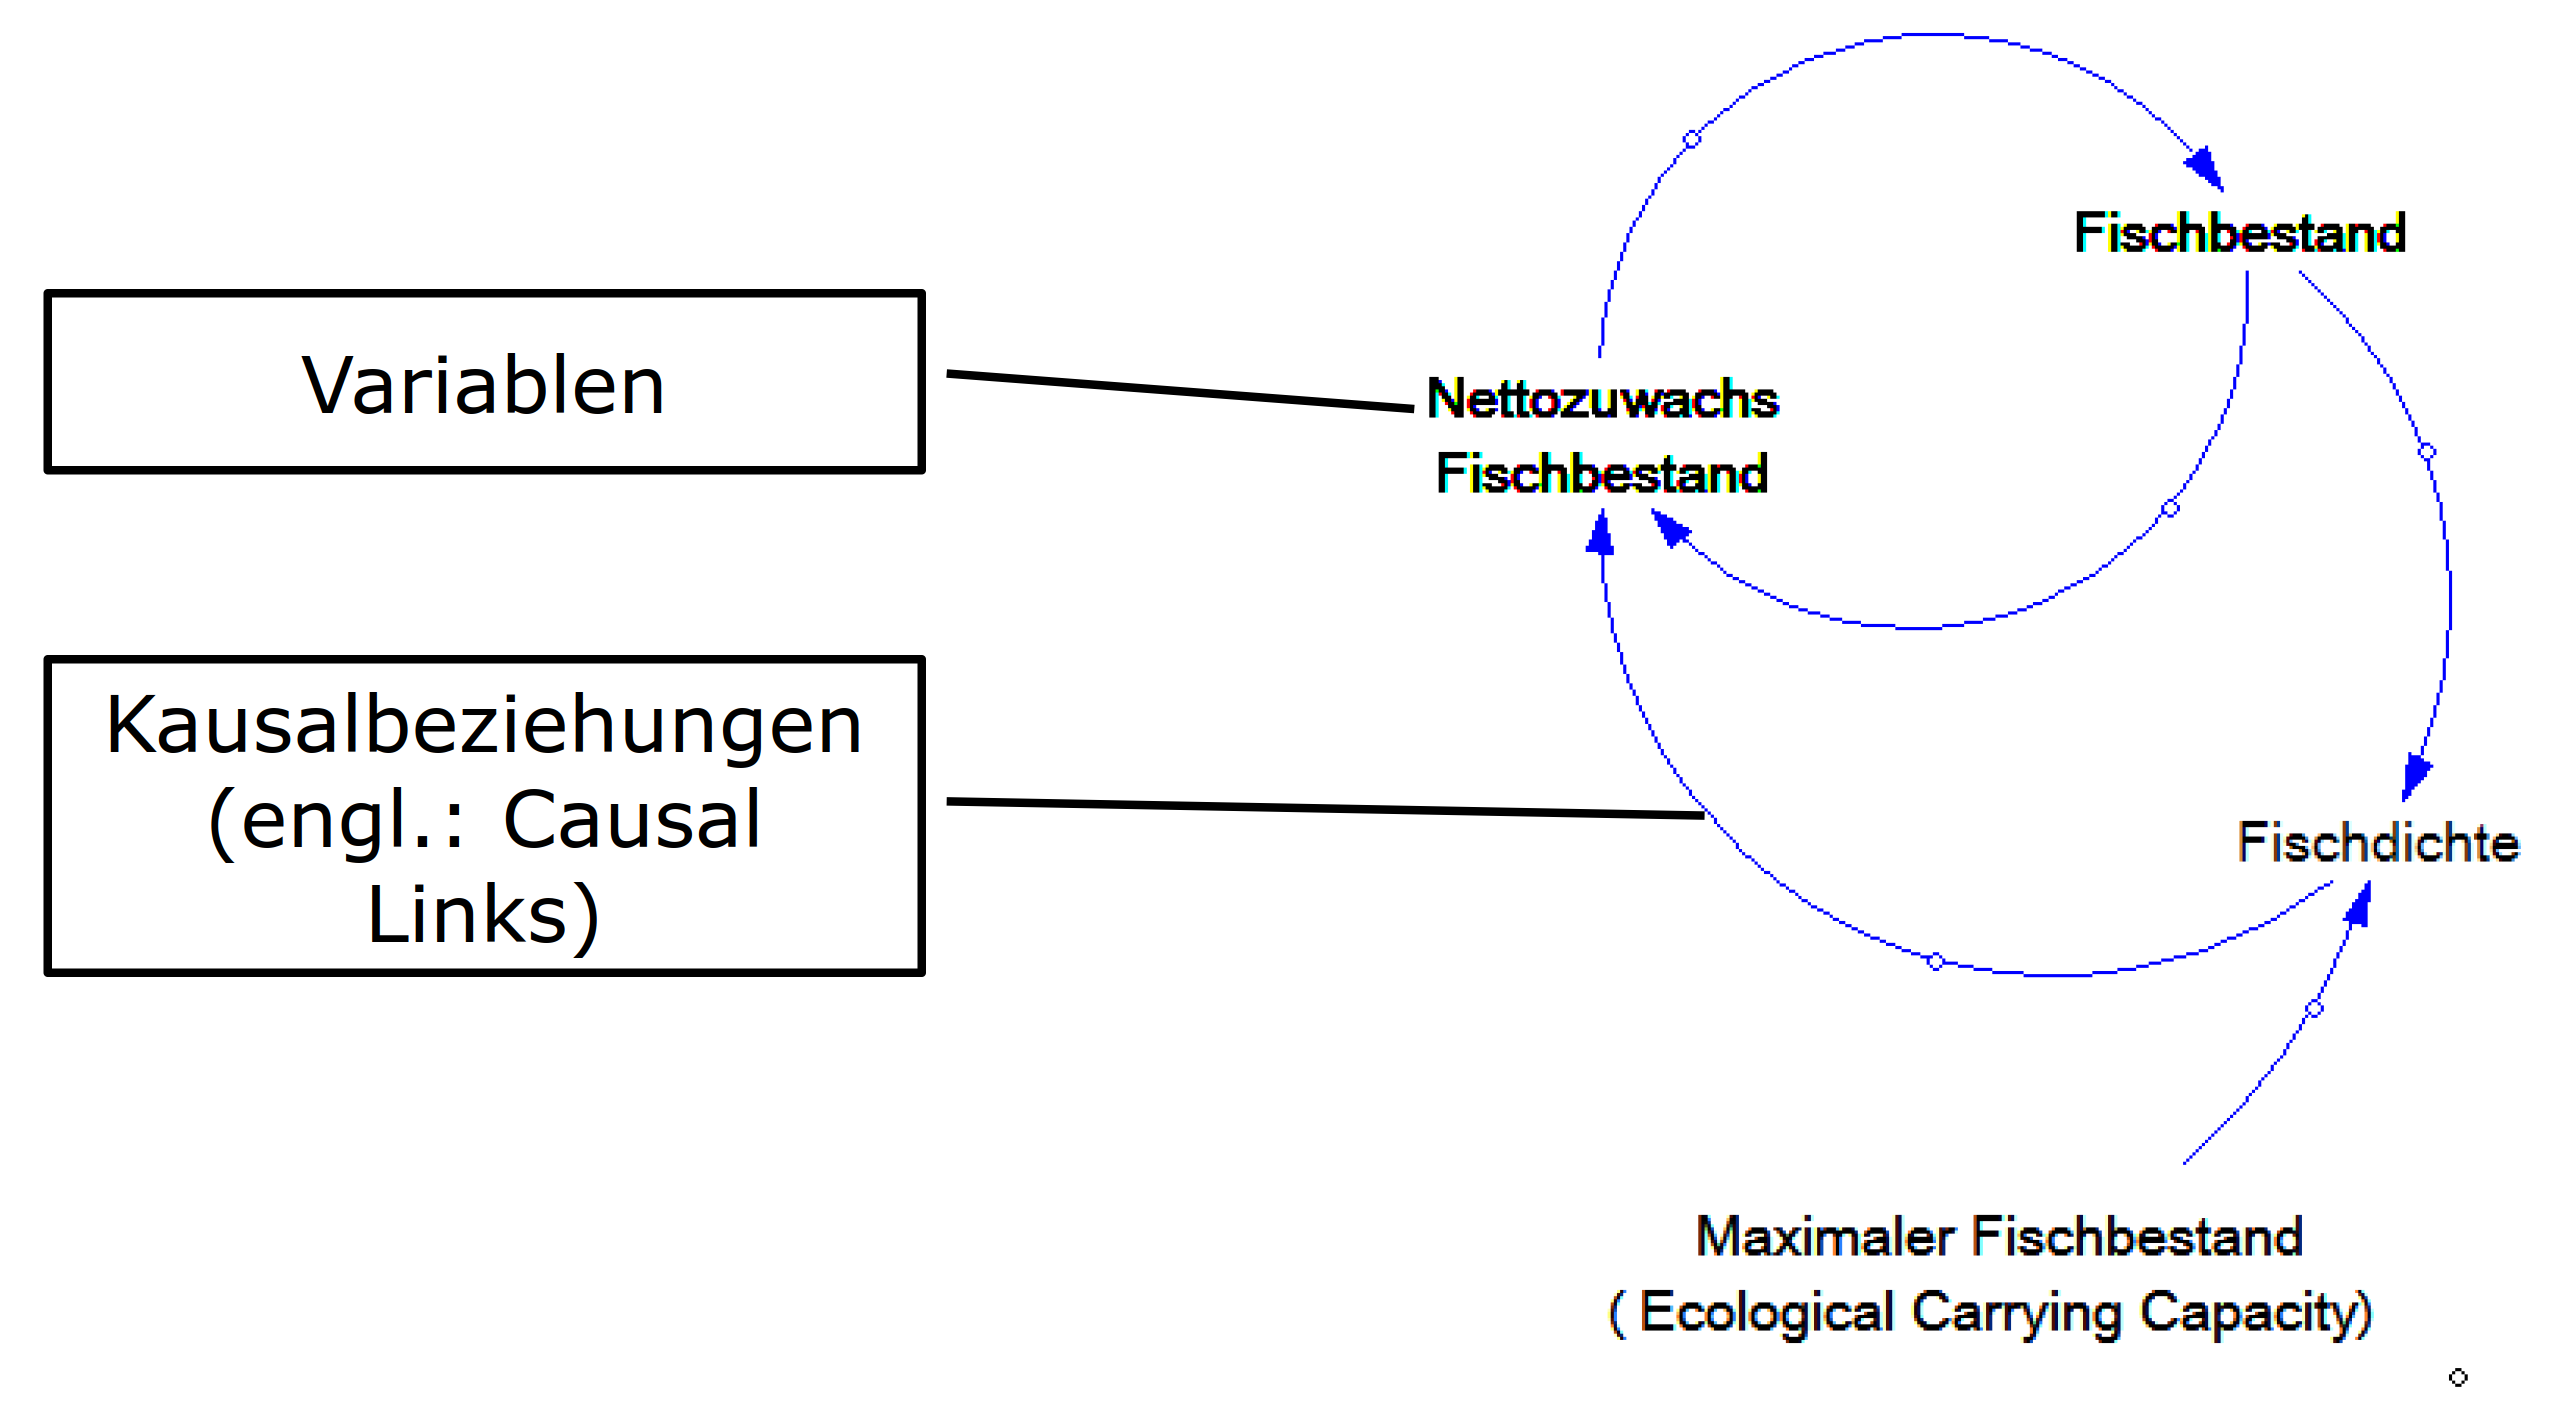
\includegraphics[width=0.5\textwidth]{pictures/kausales_modell}

	\subsubsection{Polarität einer Kausalbeziehung}
	\textbf{Positive Polarität:} Steigt (fällt) Ursache, dann steigt (fällt) Wirkung \\
	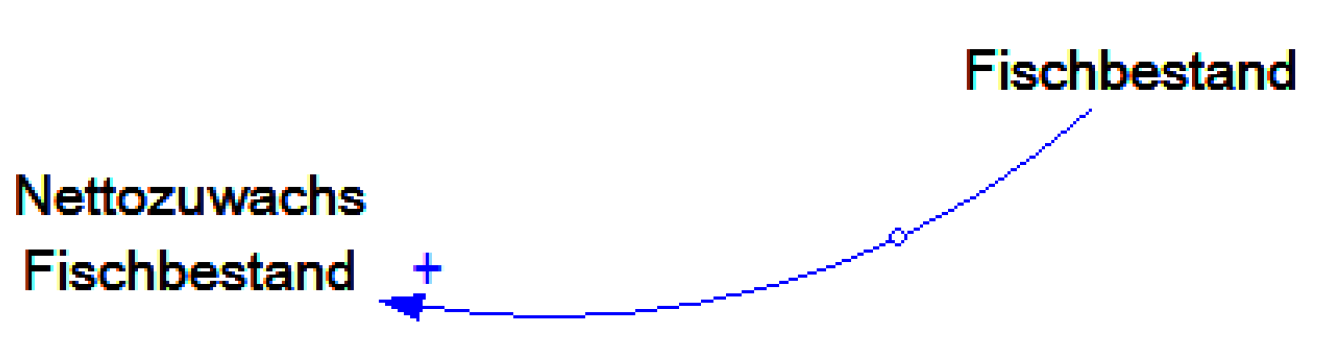
\includegraphics[width=0.35\textwidth]{pictures/positive_polaritaet}\\
	\textbf{Negative Polarität:} Steigt (fällt) Ursache, dann fällt (steigt) Wirkung \\
	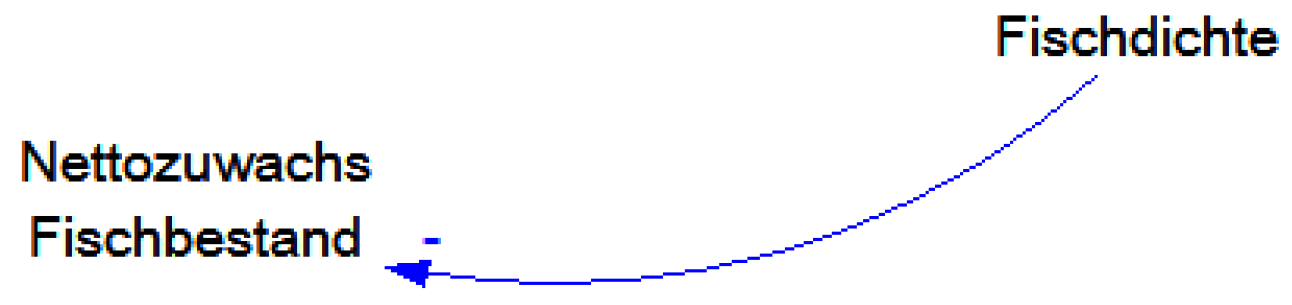
\includegraphics[width=0.35\textwidth]{pictures/negative_polaritaet}
\end{multicols}

\begin{multicols}{3}
	\subsubsection{Rückkopplung}
	Gerichteter Kreis von Kausalbeziehungen. \\
	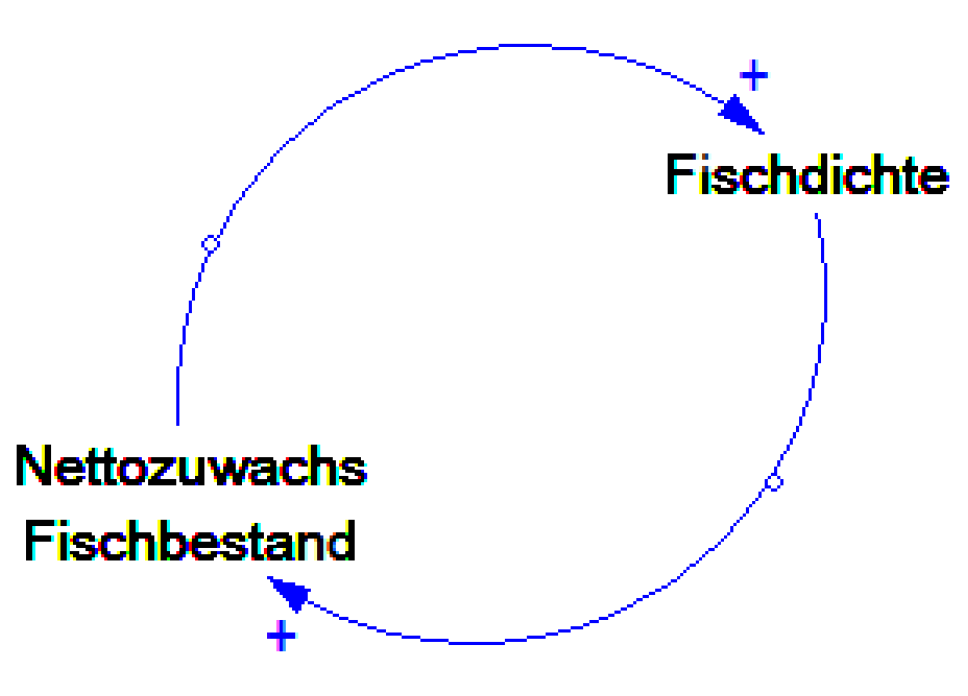
\includegraphics[width=0.25\textwidth]{pictures/rueckkopplung} \\
	
	\subsubsection{Selbstverstärkender Loop}
	Die Rückkoppelung verstärkt einen anfänglichen Effekt. \\
	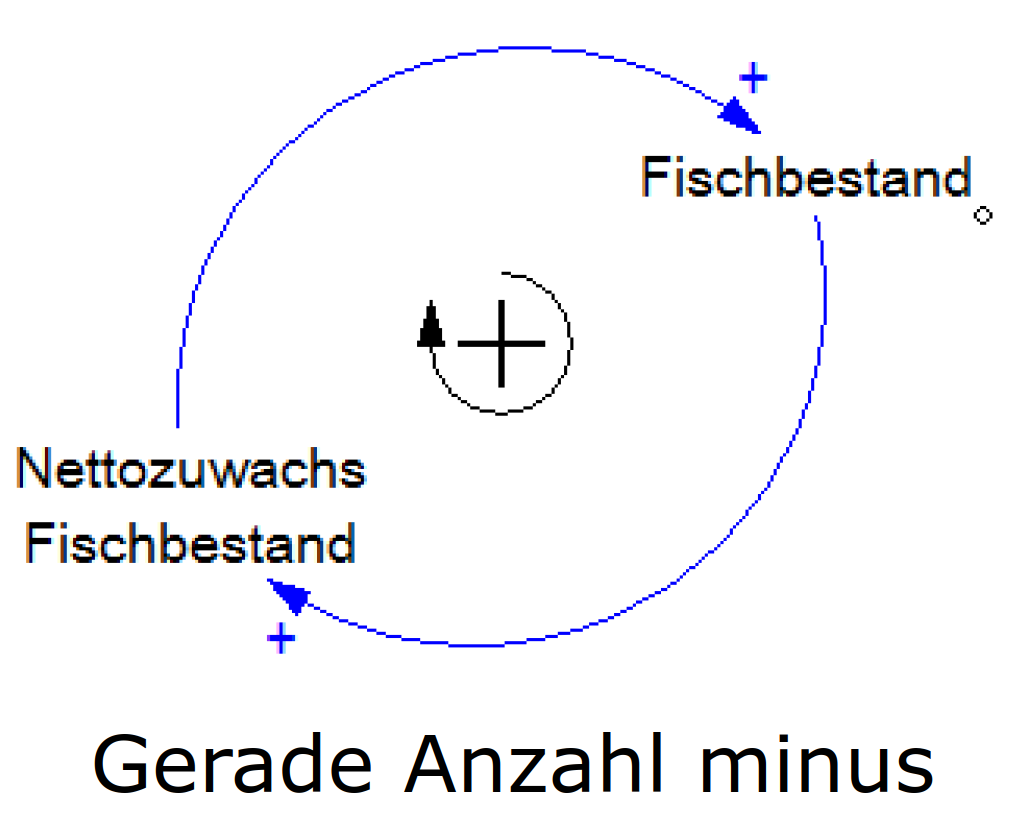
\includegraphics[width=0.25\textwidth]{pictures/selbstverstaerkender_loop}
	
	\subsubsection{Ausgleichender Loop}
	Die Rückkoppelung wirkt	einem anfänglichen Effekt entgegen.\\
	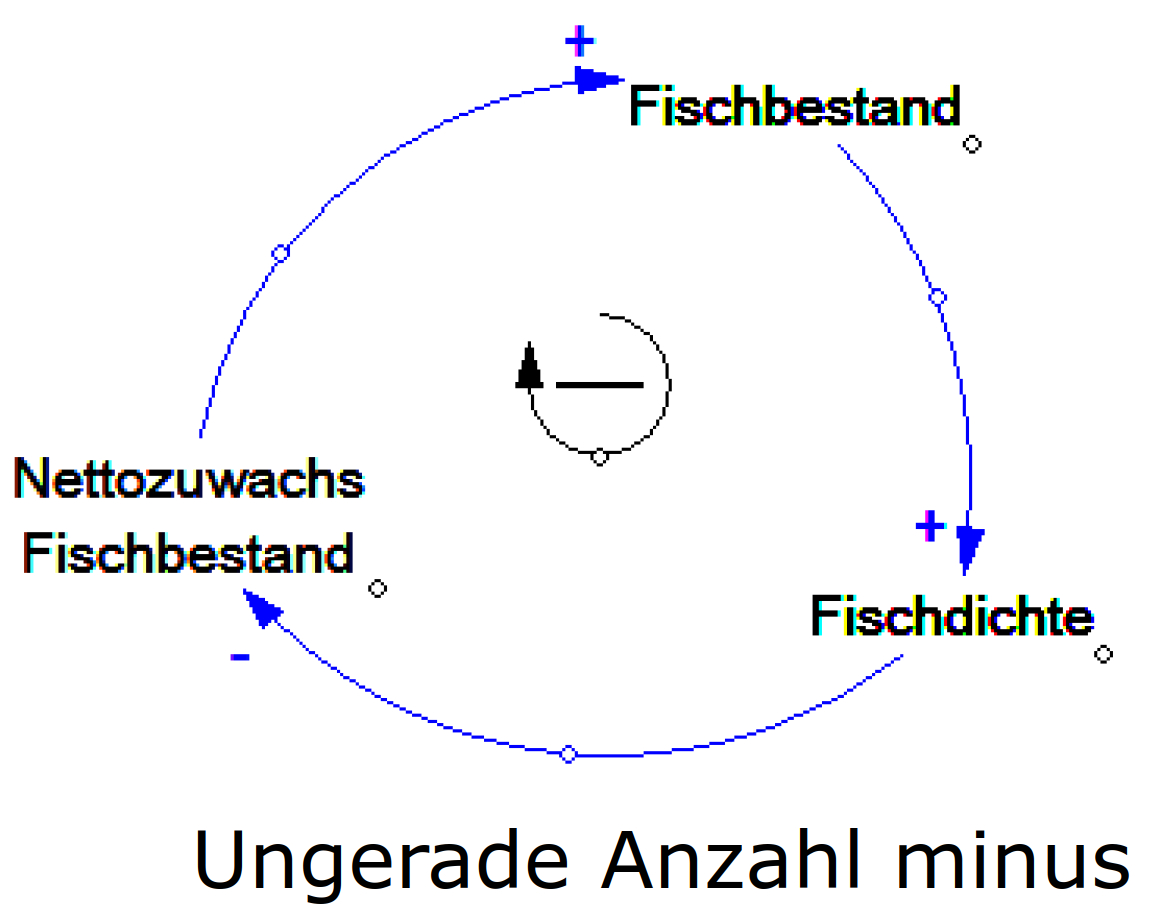
\includegraphics[width=0.25\textwidth]{pictures/ausgleichender_loop}
\end{multicols}	

\begin{multicols}{2}
	\subsubsection{Stock-and-Flow Diagramm}
	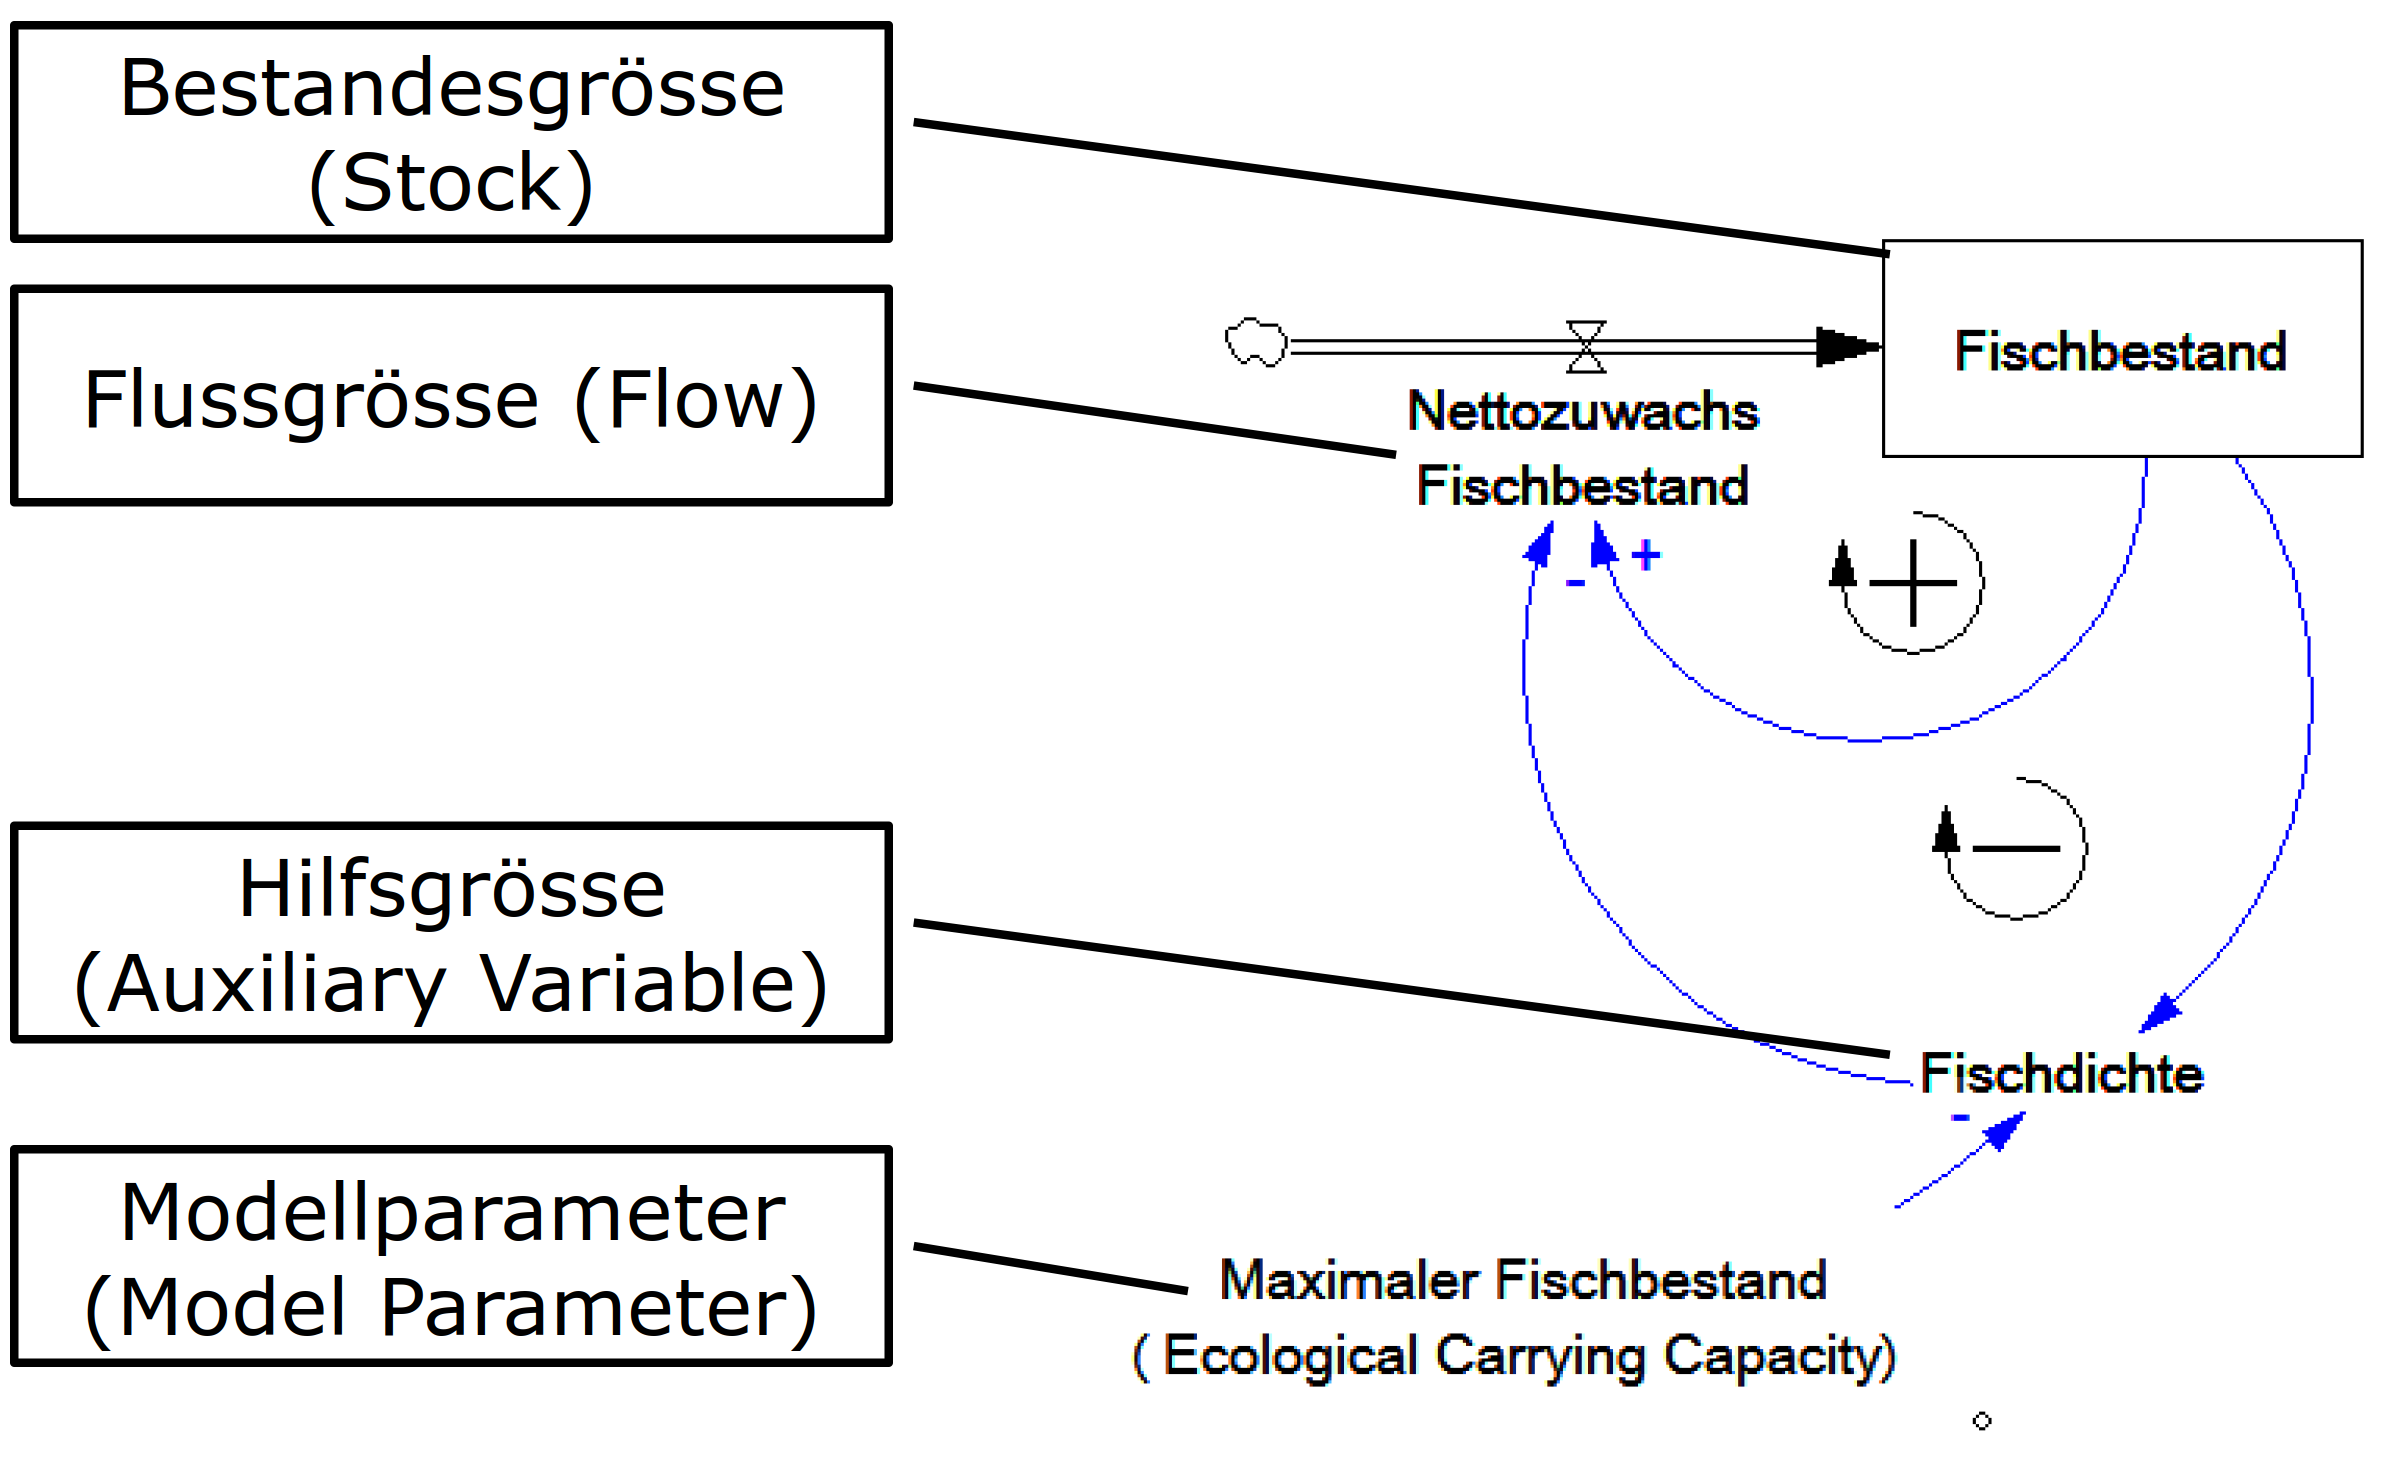
\includegraphics[width=0.5\textwidth]{pictures/stock_and_flow_diagramm}
	
	\subsubsection{Systemdynamisches Simulationsmodell}
	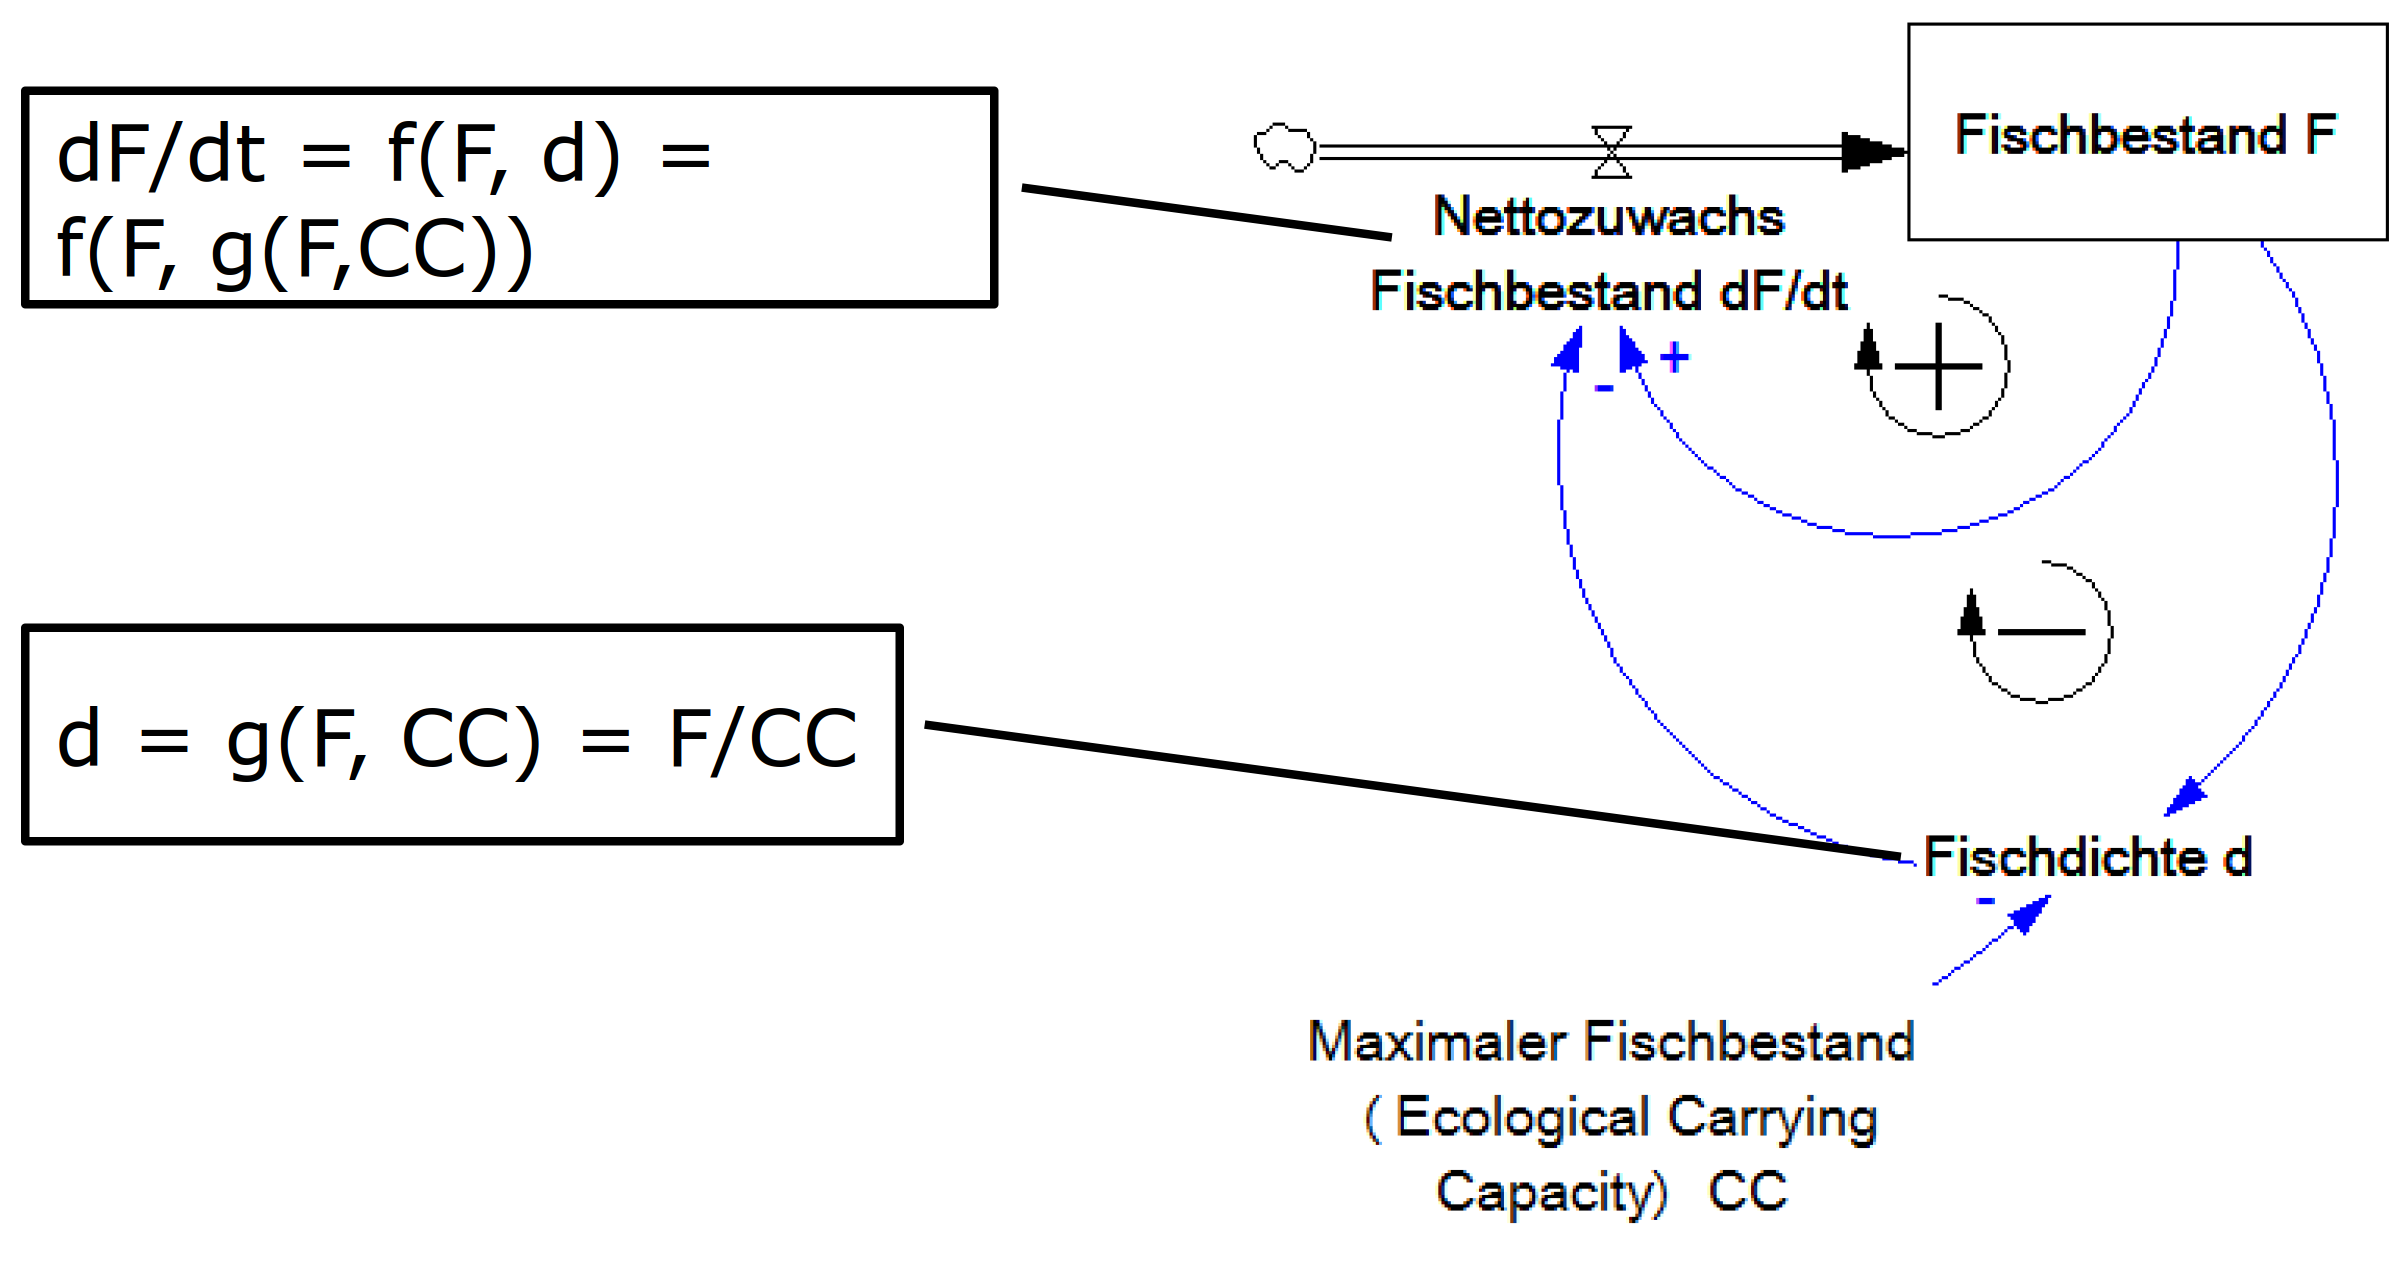
\includegraphics[width=0.5\textwidth]{pictures/systemdynamisches_simulationsmodell}
\end{multicols}	

\subsection{Grundideen}
\subsubsection{Ziele}
\begin{compactitem}
	\item \textbf{Verständnis, nicht Prognose} \\
	The goal of a system dynamics policy study is understanding - understanding the interactions in a complex system that are 	conspiring to create a problem, and understanding the structure	and dynamic implications of policy changes intended to improve	the system's behaviour (Richardson 1991: 164)
	\item \textbf{Modellieren, um zu lernen} \\
	Therefore, the primary goal is not to build the model of the system, but rather to get a group engaged in building a system dynamics model of a problem in order to see to what	extent this process might be helpful to increase problem understanding and to devise courses of action to which team members feel committed (Vennix 1996: 3).
\end{compactitem}

\subsubsection{Darstellungsformen}
\begin{compactenum}
	\item \textbf{Causal Loop Diagramme (\aszeichen{Kausaldiagramme})}
	\begin{compactitem}
		\item Kommunikations-Tool für ein gemeinsames mentales Modell und generelle Diskussionen
	\end{compactitem}
	\item \textbf{Stock-and-Flow Diagramme (\aszeichen{Flussdiagramme})}
	\begin{compactitem}
		\item Präzise Darstellung von Lagern (Stocks) und Raten (Flows)
	\end{compactitem}
	\item \textbf{Stock-and-Flow Diagramme mit Formeln}
	\begin{compactitem}
		\item Formulierung sämtlicher Flüsse als Formeln
		\item Erlaubt quantitative Simulation
	\end{compactitem}
\end{compactenum}

\subsubsection{Computersimulation}
\begin{compactitem}
	\item Die Dynamik von Feedbackmodellen korrekt interpretieren
	\item Nicht antizipierte Nebenwirkungen entdecken
	\item Modellanalyse
	\begin{compactitem}
		\item Sensitivitätsanalyse von Parametern und funktionalen Beziehungen
		\item Einfluss unterschiedlicher Modellformulierungen
		\item Massnahmenanalyse (Policy Analysis)
	\end{compactitem}
\end{compactitem}

\subsection{Akkumulation}
Grundlage zum Verstehen von Spät- und Rückwirkungen. Akkumulation zu verstehen ist eine Voraussetzung, um Systemverhalten zu verstehen.

\subsubsection{Definitionen}
Der Verlauf einer Bestandesgrösse über die Zeit ist durch die untenstehende hydraulische Metapher definiert - bzw. durch die equivalenten mathematischen Definitionen.\\
\begin{multicols}{2}
	\textbf{Bestandes- und Flussdiagramm (Stock-and-Flow-Diagramm):} \\
	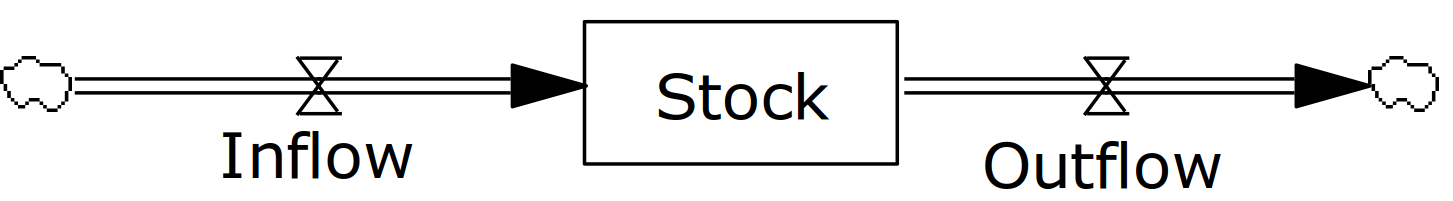
\includegraphics[width=0.5\textwidth]{pictures/badewanne_stock} \\
	\textbf{Integralgleichung:} \\
	$Stock(t) = \integral{t_0}{t}{[Inflow(s)-Outflow(s)]}{s}+Stock(t_0)$\\
	\textbf{Differentialgleichung:} \\
	$\differential{Stock(t)}{t} = Inflow(t) - Outflow(t)$ \\
	\textbf{Metapher aus der Hydraulik:} \\
	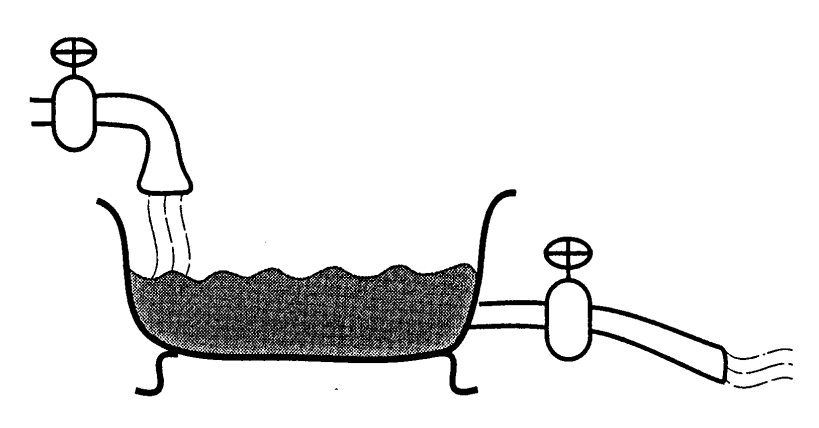
\includegraphics[width=0.35\textwidth]{pictures/badewanne}
\end{multicols}

\begin{multicols}{2}
	\subsubsection{Bestandesgrössen (Stocks)}
	\begin{compactitem}
		\item sind Zustandsgrössen, die “Erinnerung” eines Systems
		\item müssen mit einem Anfangswert charakterisiert werden
		\item ändern sich ausschliesslich durch Zu- und Abfluss
		\item Wert verändert sich nicht \textless-\textgreater\ Zufluss = Abfluss
		\item Wert wächst \textless-\textgreater\ Zufluss \textgreater\ Abfluss
		\item Wert fällt \textless-\textgreater\ Zufluss \textless\ Abfluss
		\item haben Masseinheiten wie Liter, CHF, Meter
	\end{compactitem}
	
	\subsubsection{Flussgrössen (Flows)}
	\begin{compactitem}
		\item sind Änderungsraten von Bestandesgrössen
		\item haben Masseinheiten wie Liter/Stunde, CHF/Jahr, Meter/Sekunde
	\end{compactitem} \ \\ \ \\ \ \\
\end{multicols}

\subsection{Causal Loop Diagramme}
\subsubsection{Vergleich CLD und Stock-and-Flow Diagramm}
\begin{multicols}{2}
	\textbf{Stock-and-Flow Diagramm:} \\
	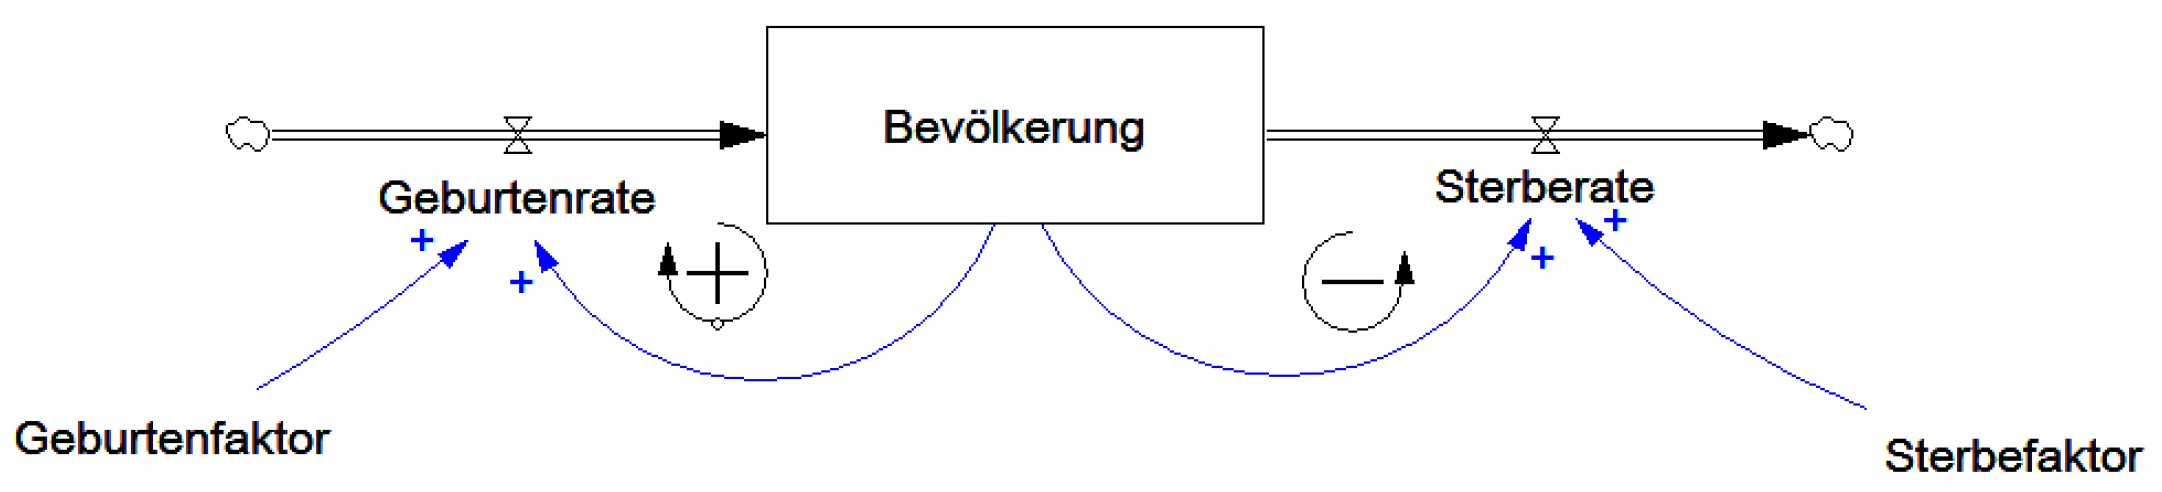
\includegraphics[width=0.5\textwidth]{pictures/vergleich_stock} \\ \\
	\textbf{Causal Loop Diagramm:} \\
	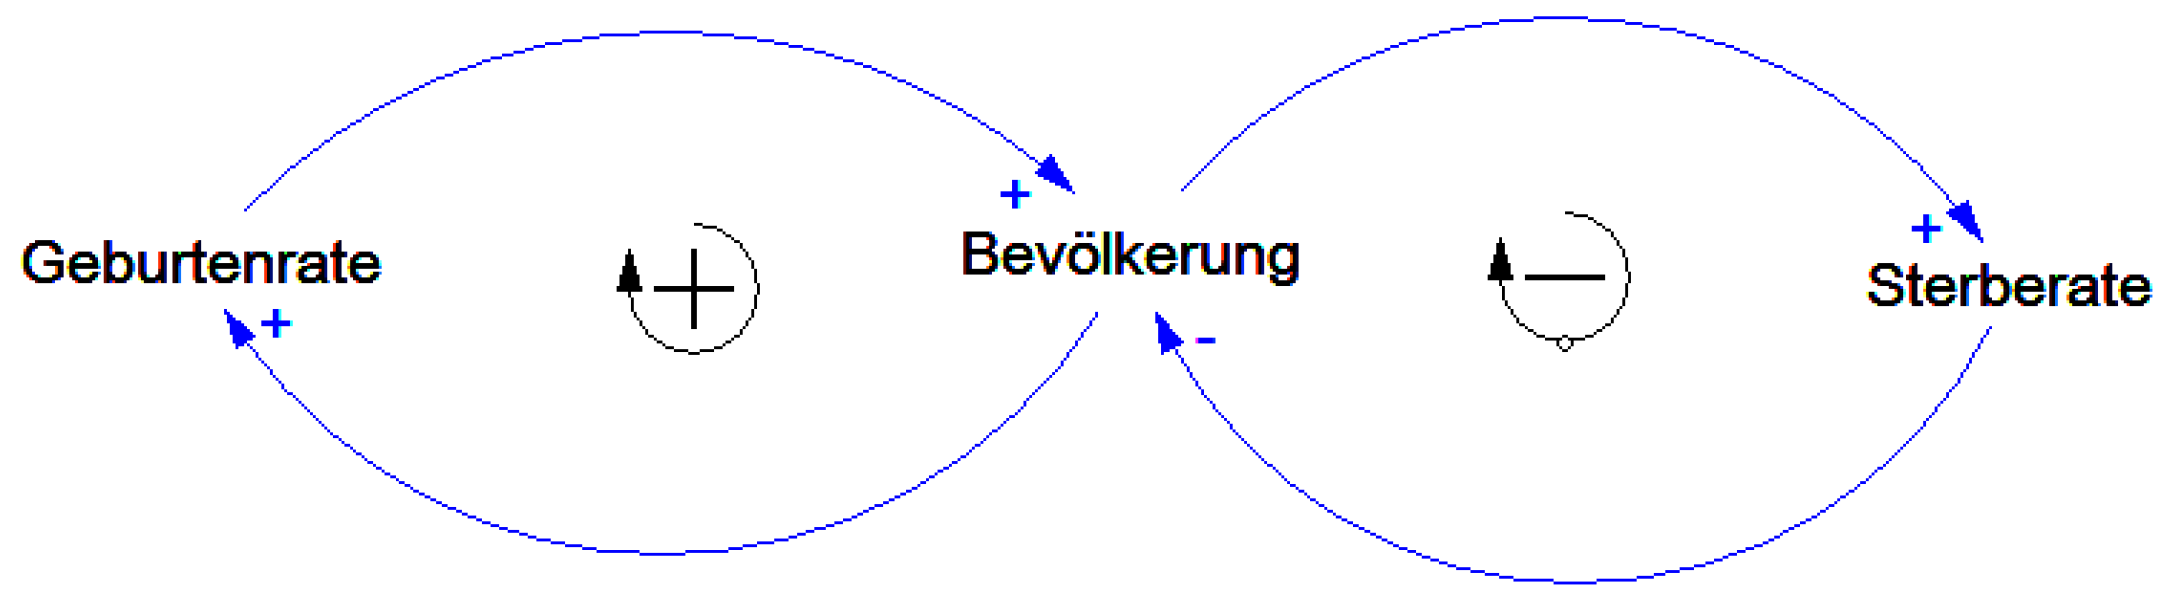
\includegraphics[width=0.5\textwidth]{pictures/vergleich_cld} 
\end{multicols}	

\subsubsection{Unmittelbare und akkumulierende Kausalbeziehungen}
Werden im CLD graphisch nicht unterschieden.
\begin{multicols}{2}
	\textbf{Unmittelbar:} \\
	Steigt (fällt) A, dann steigt (fällt) B \\
	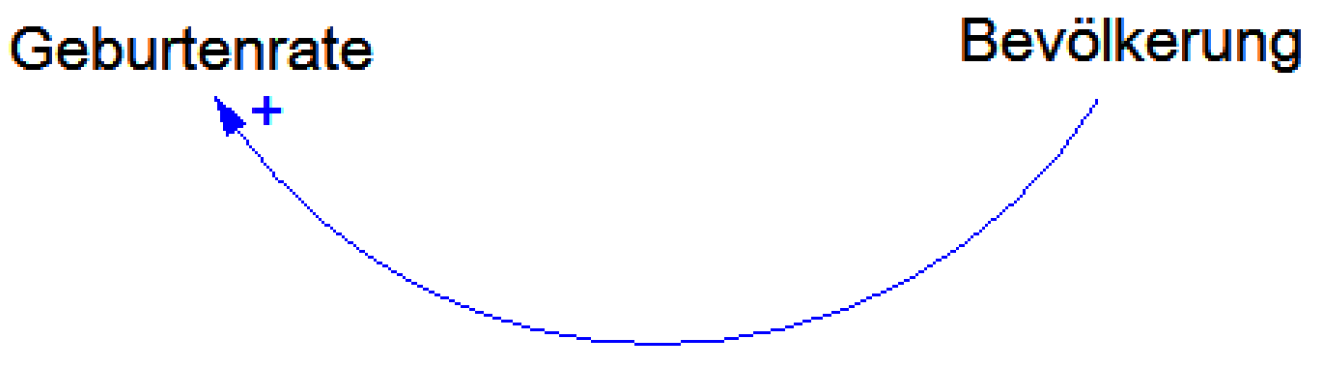
\includegraphics[width=0.35\textwidth]{pictures/unmittelbar_1} \\
	Steigt (fällt) A, dann fällt (steigt) B \\
	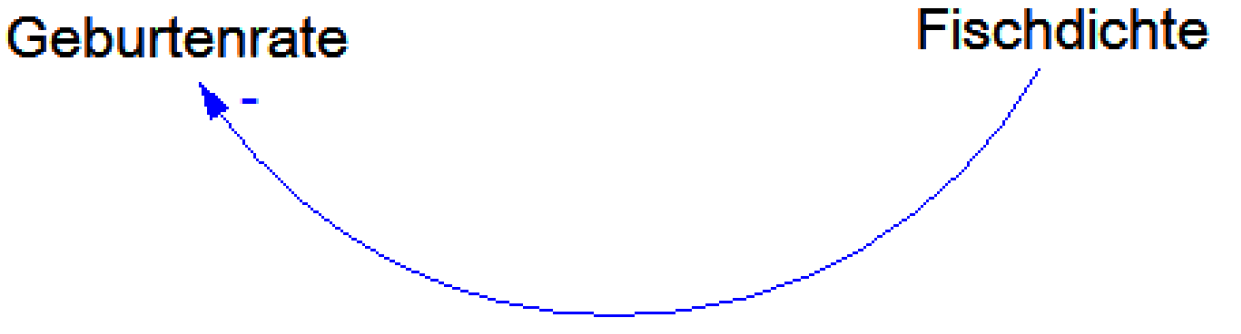
\includegraphics[width=0.35\textwidth]{pictures/unmittelbar_2} \\
	\textbf{Akkumulierend:} \\
	A wird zu B addiert, $B=\integral{t_0}{t}{A}{d}+A_0$\\
	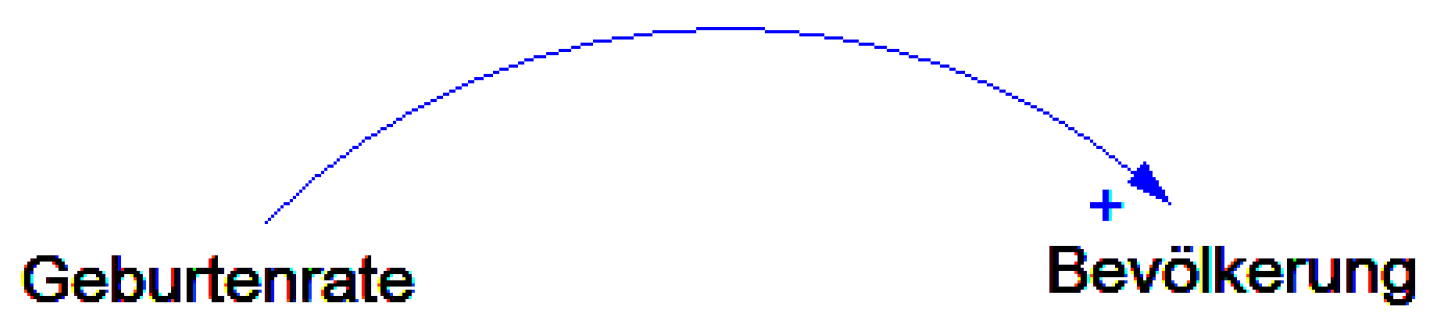
\includegraphics[width=0.35\textwidth]{pictures/akkumulierend_1} \\
	A wird von B subtrahiert, $B=\integral{t_0}{t}{-A}{d}+A_0$\\
	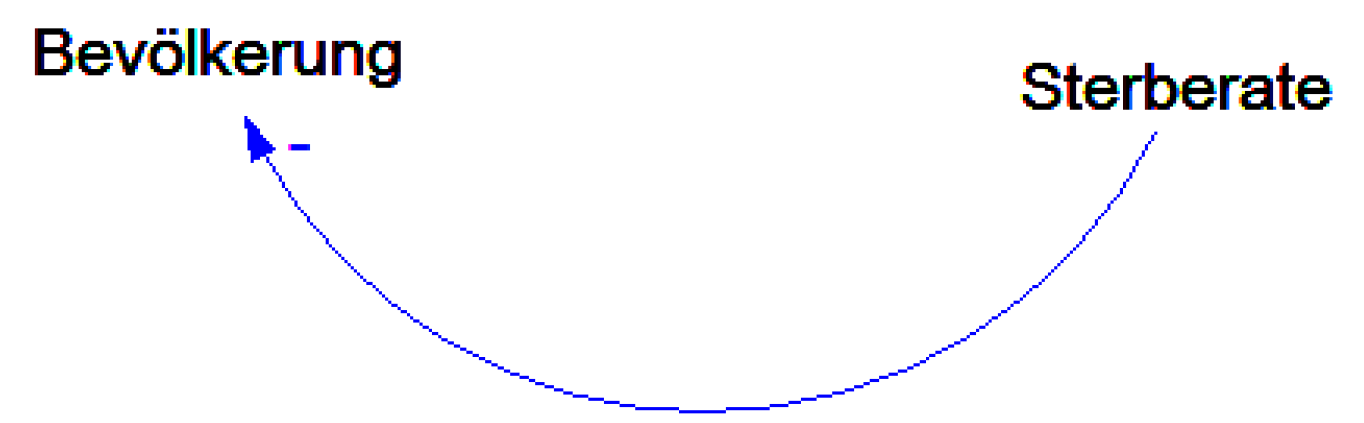
\includegraphics[width=0.35\textwidth]{pictures/akkumulierend_2}
\end{multicols}	

\subsubsection{Möglichkeiten}
\begin{compactitem}
	\item sich in einem komplexen System Übersicht verschaffen, System verstehen
	\item Steuermöglichkeiten (\aszeichen{Stellhebel}) erkennen
	\item Suche nach Neben- und Rückwirkungen von scheinbar zielführenden Massnahmen erleichtern
	\item Zielgrössen identifizieren, Zielkonflikte offen legen
	\item Diskussionsqualität verbessern: präzise erklären, wovon die Rede ist
\end{compactitem}

\newpage

\subsubsection{Regeln für gute CLDs}
\begin{multicols}{2}
	\begin{compactenum}
		\item (Variablennamen) Substantive als Variablennamen wählen
		\item (Variablennamen) Keine Richtung der Dynamik durch Variablennamen vorgeben \\
		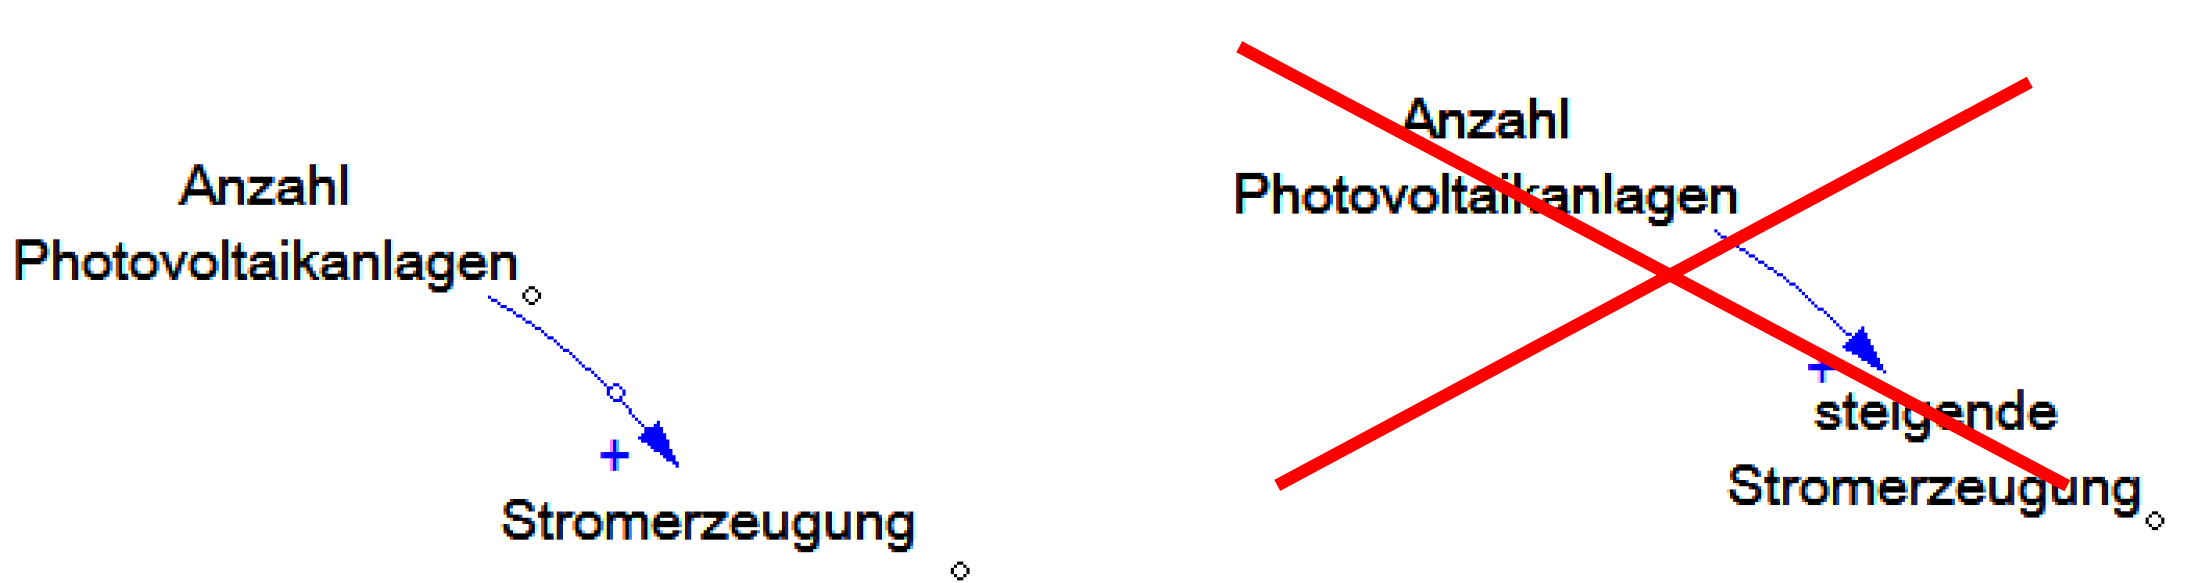
\includegraphics[width=0.45\textwidth]{pictures/regel_2}
		\item (Variablennamen) Der Wert von Variablen muss grösser oder kleiner werden können - der Name bezeichnet im Idealfall ein Kontinuum \\
		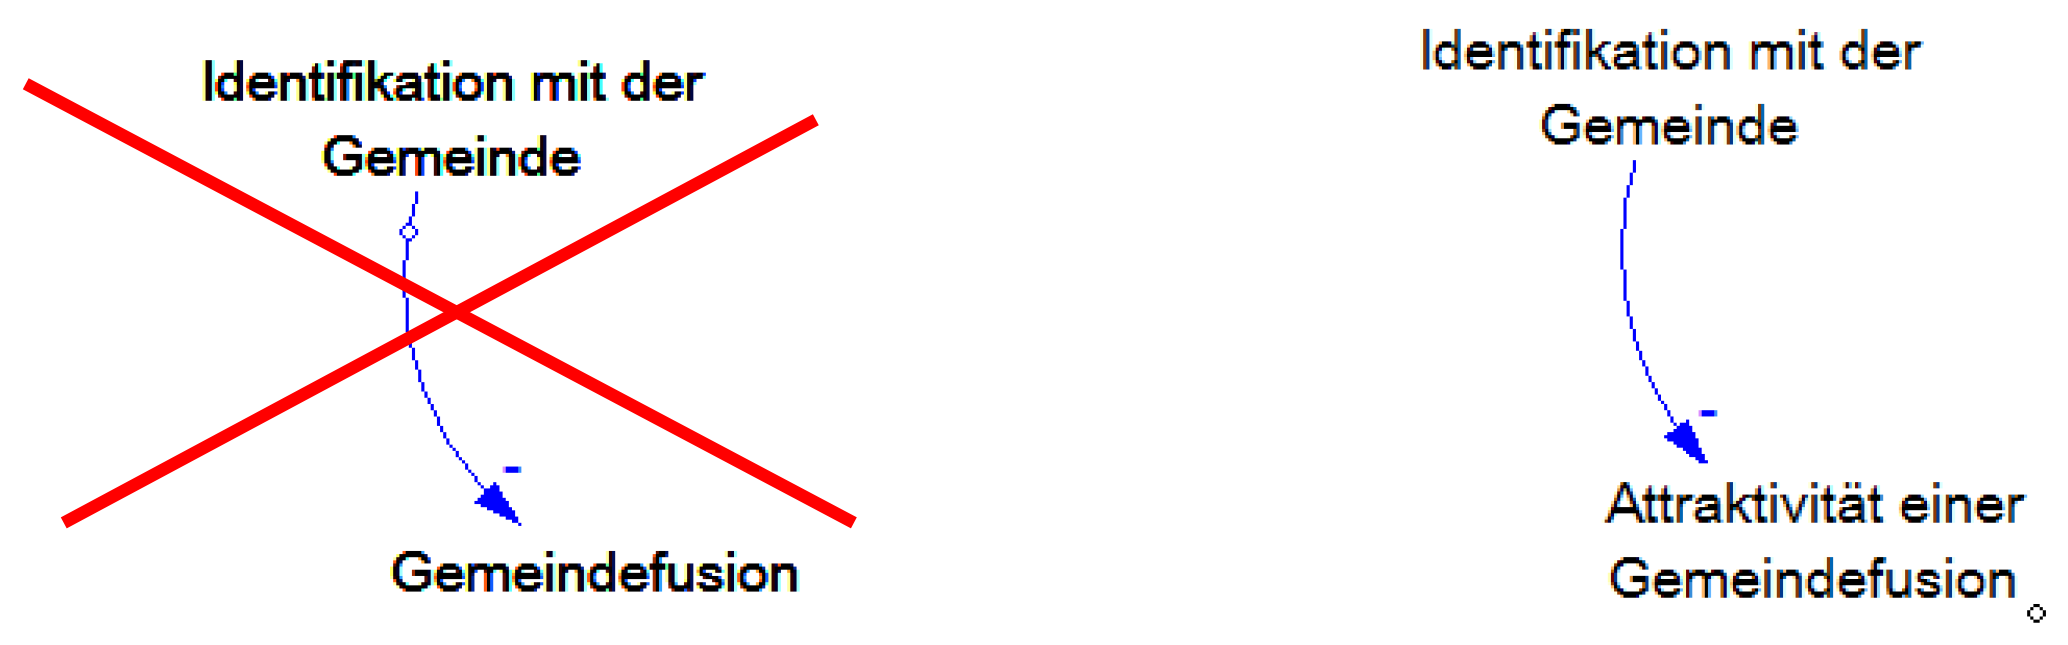
\includegraphics[width=0.45\textwidth]{pictures/regel_3}
		\item (Kausalbeziehungen) Kausalität, nicht Korrelation modellieren
		\begin{compactitem}
			\item Nur Kausalitäten aufzeichnen, die Sie überzeugen
			\item Relevante kausale Erklärungen zu finden, ist ein kreativer Akt und erfordert den Austausch zwischen den beteiligten Personen (Statistik	reicht nicht)
		\end{compactitem}
		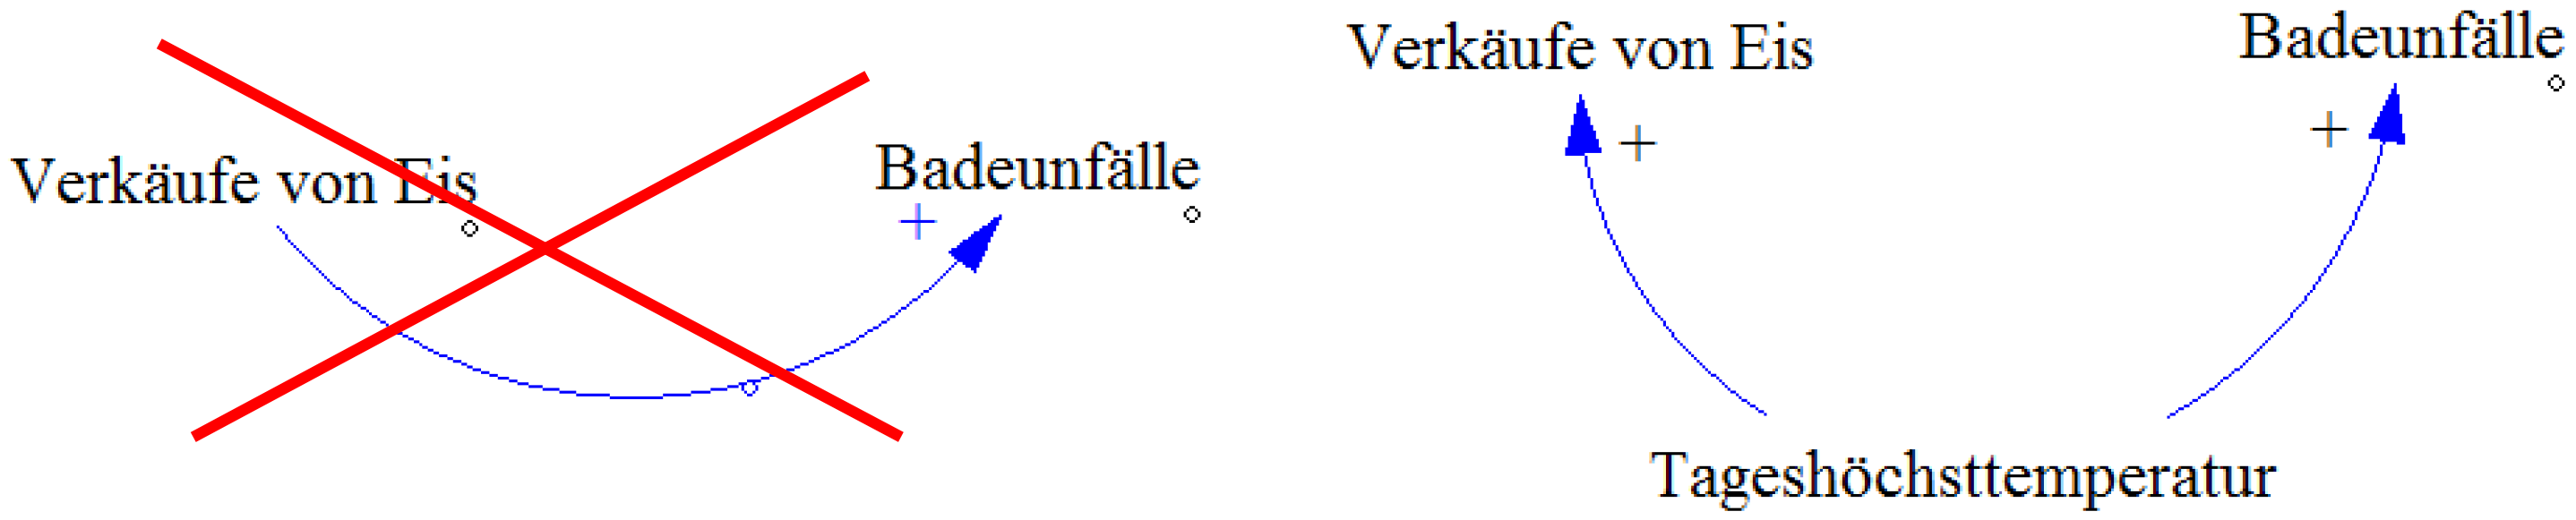
\includegraphics[width=0.45\textwidth]{pictures/regel_4}
		\item (Kausalbeziehungen) Kausalbeziehungen mit eindeutiger Polarität modellieren: Ist keine Polarität zuweisbar ist, dann muss die	Kausalbeziehung, bzw. unterliegende Struktur besser	analysiert werden. \\
		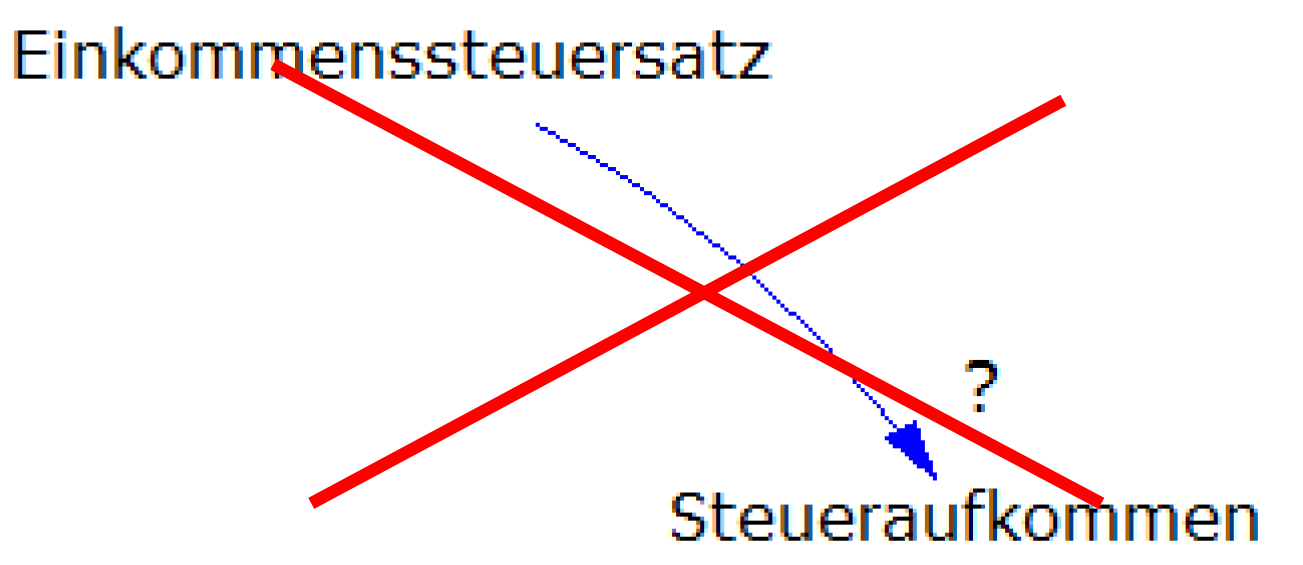
\includegraphics[width=0.225\textwidth]{pictures/regel_5} 
		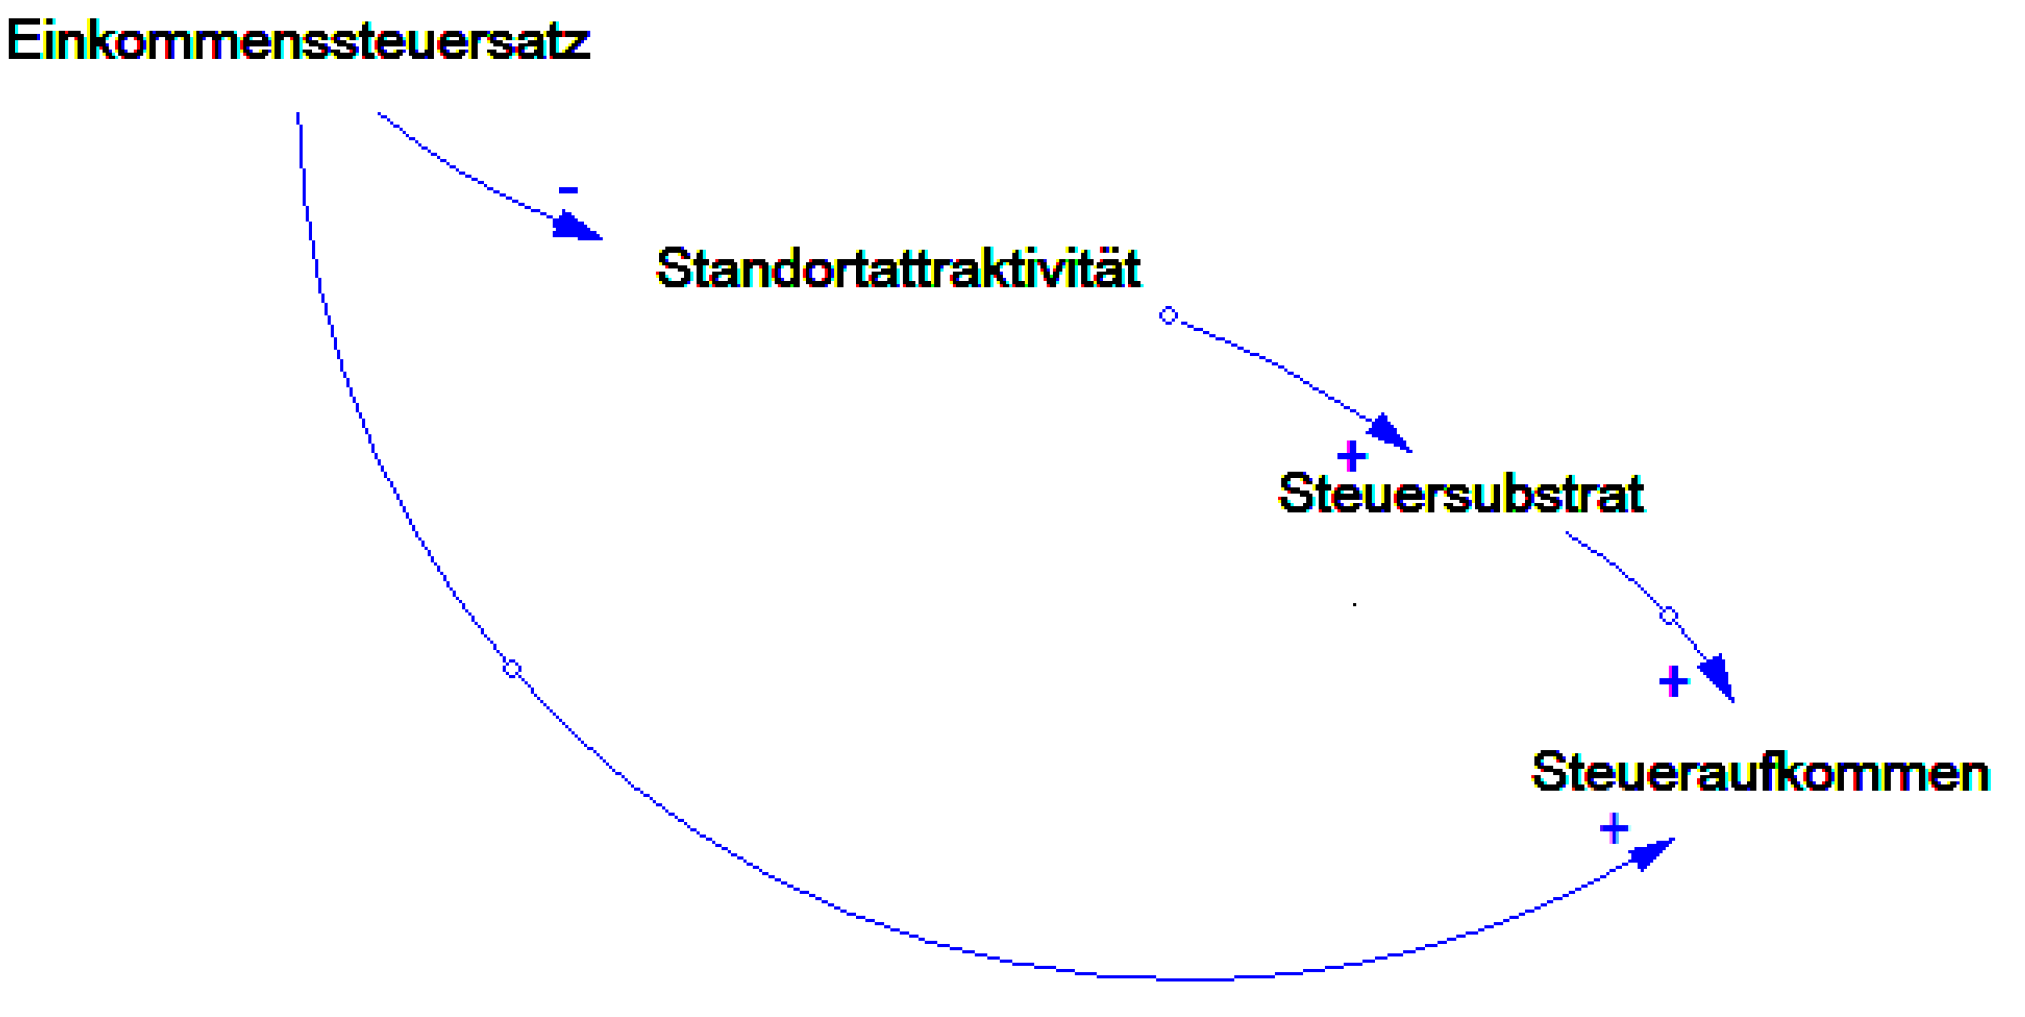
\includegraphics[width=0.225\textwidth]{pictures/regel_5_2}
		\item (Kausalbeziehungen) Kein \aszeichen{Einkaufszettel} (Daumenregel: max. 3 Ursachen für	eine Wirkung) \\
		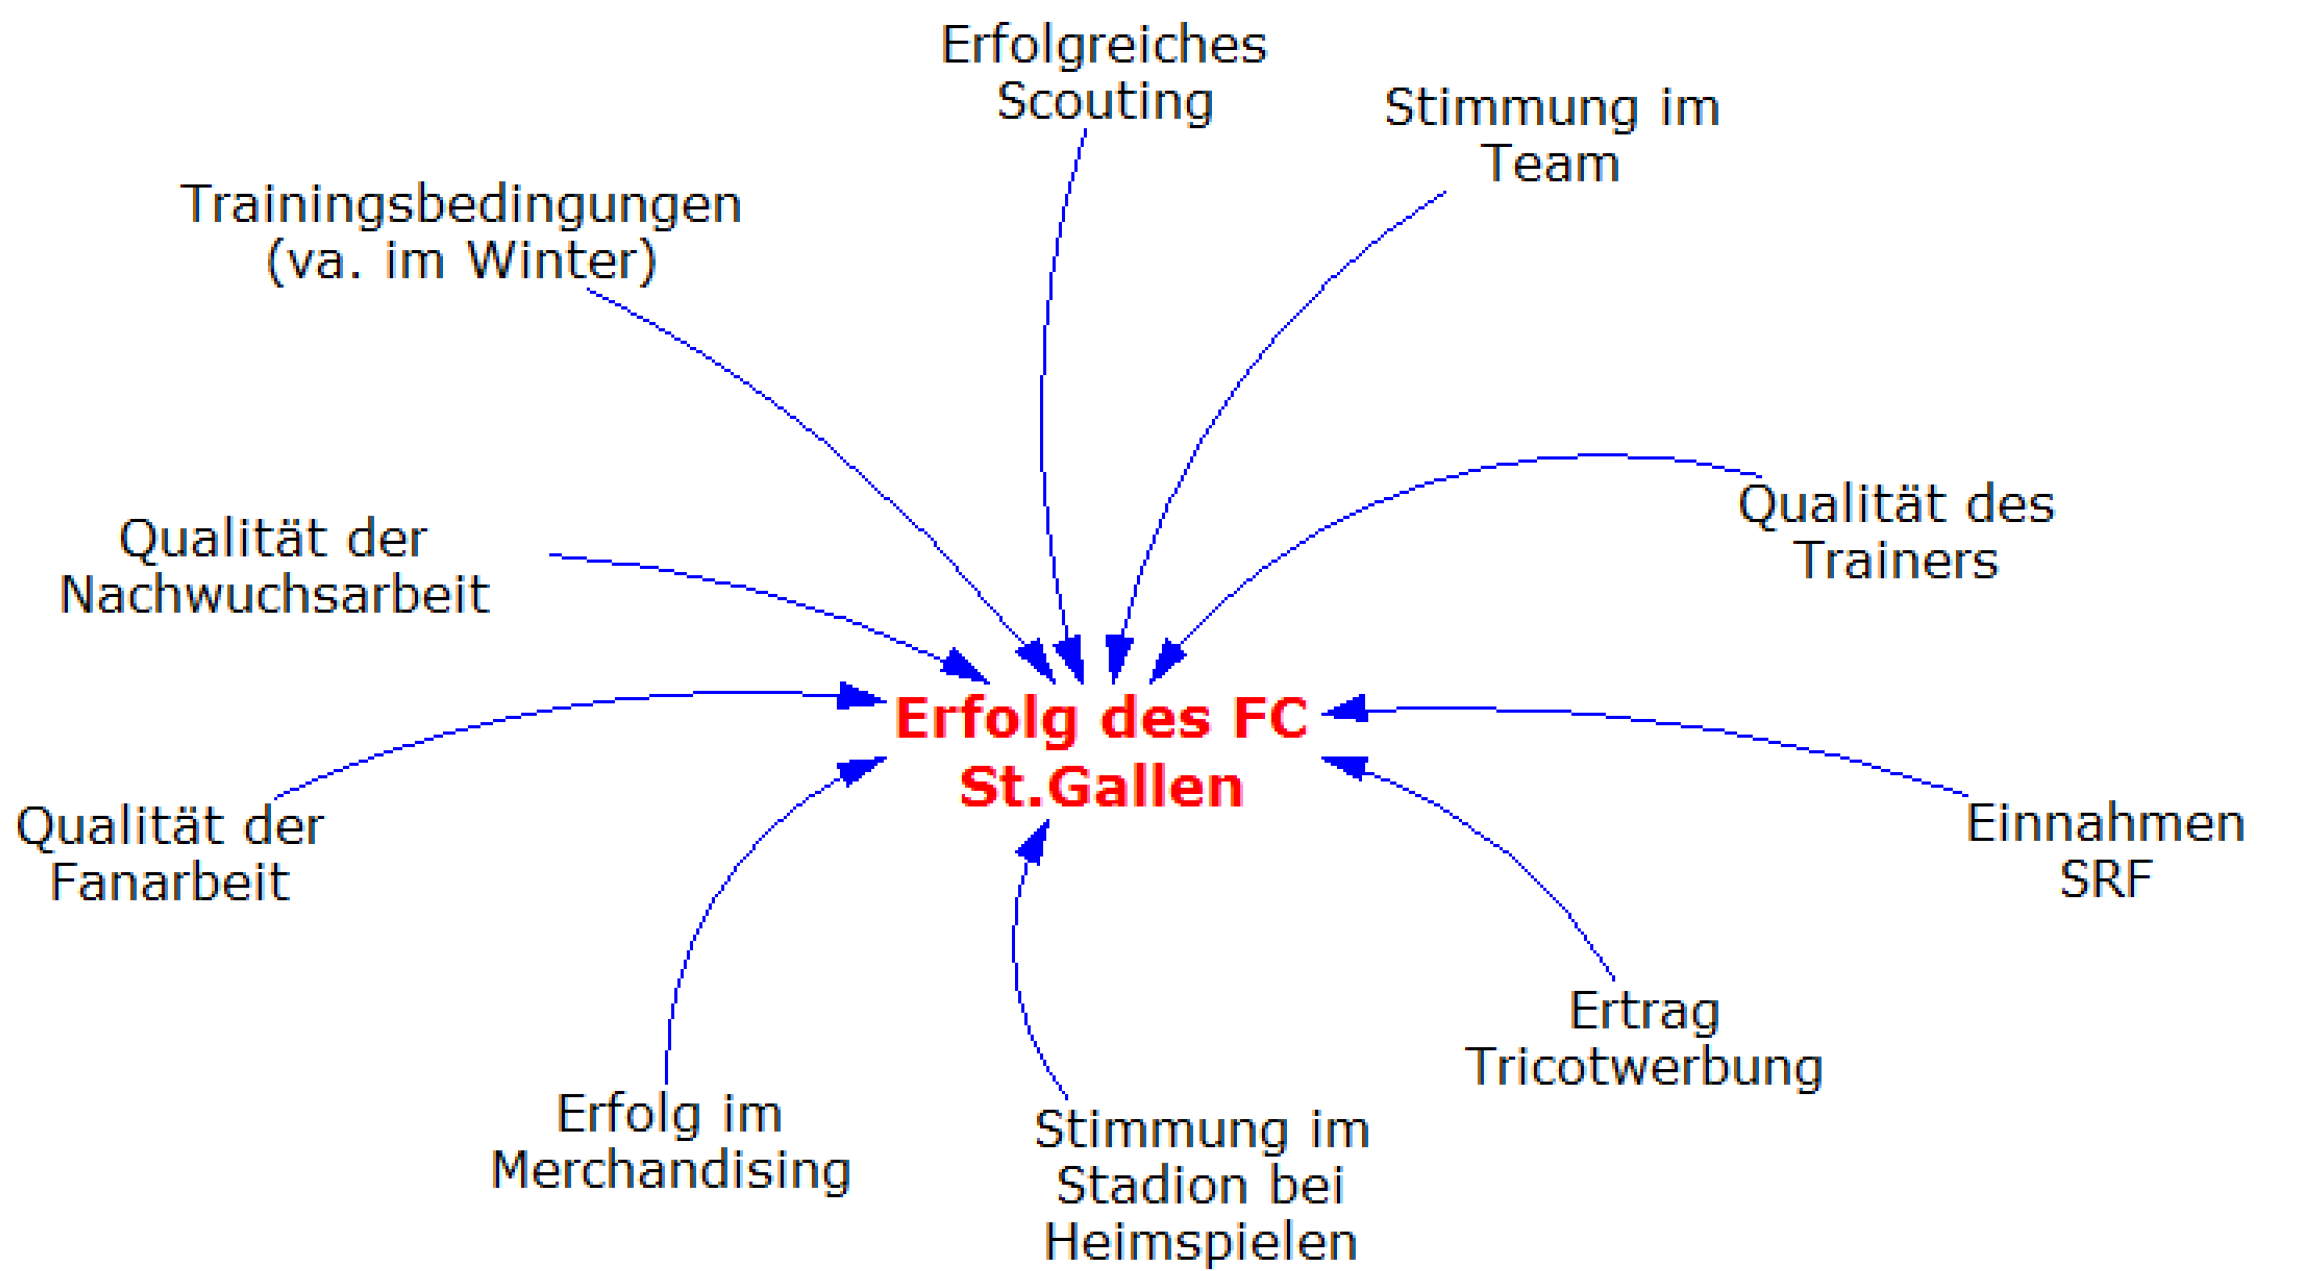
\includegraphics[width=0.45\textwidth]{pictures/regel_6} \\ \\ \\ \\ \\
		\item (Kausalbeziehungen) Vermeiden Sie Redundanz \\
		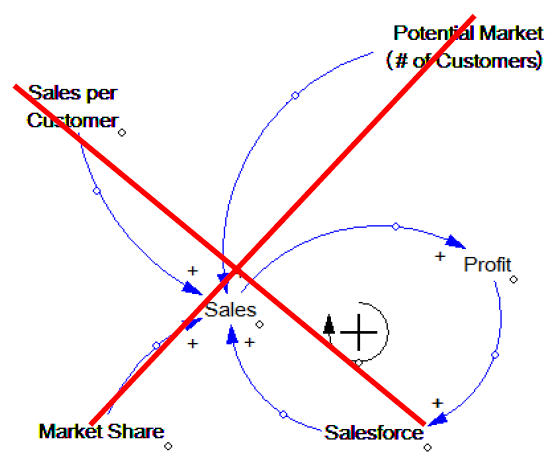
\includegraphics[width=0.225\textwidth]{pictures/regel_7} 
		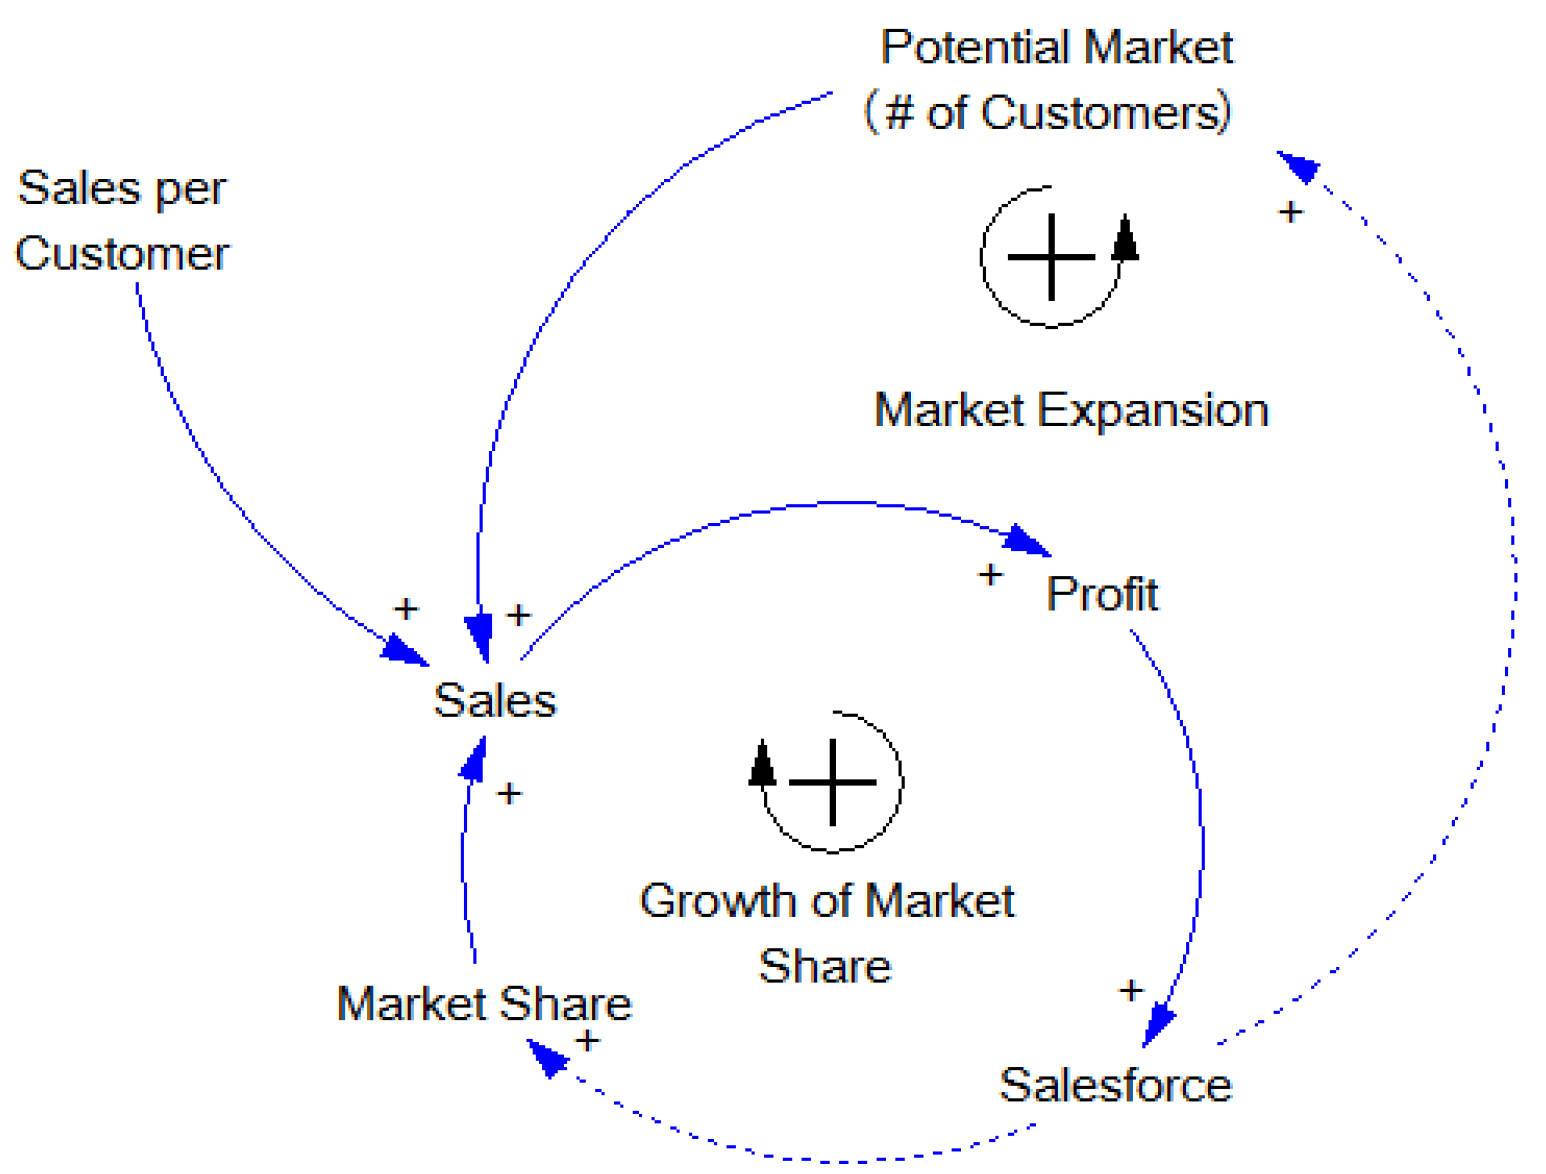
\includegraphics[width=0.225\textwidth]{pictures/regel_7_2}
		\item (Kausalbeziehungen) Stellen Sie bei jeder Entscheidungsregel die Frage: Gibt es auch unerwünschte Wirkungen? \\
		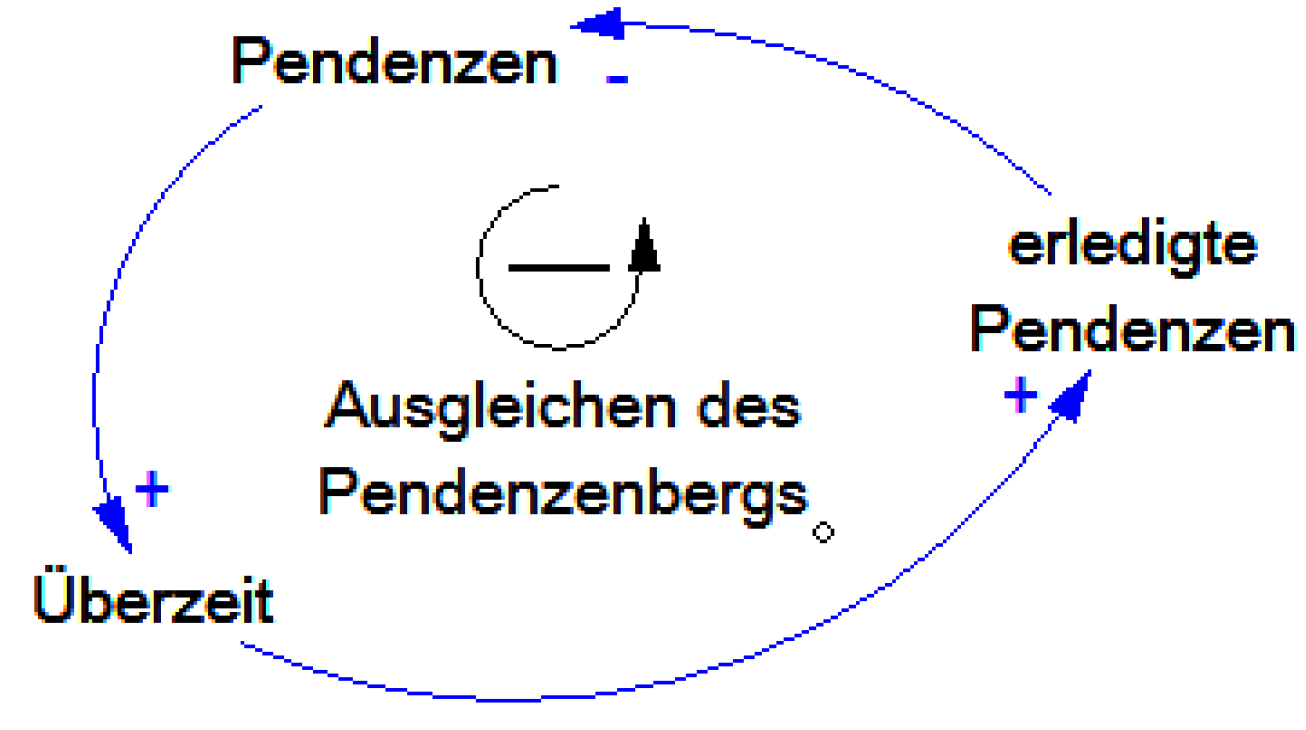
\includegraphics[width=0.225\textwidth]{pictures/regel_8} 
		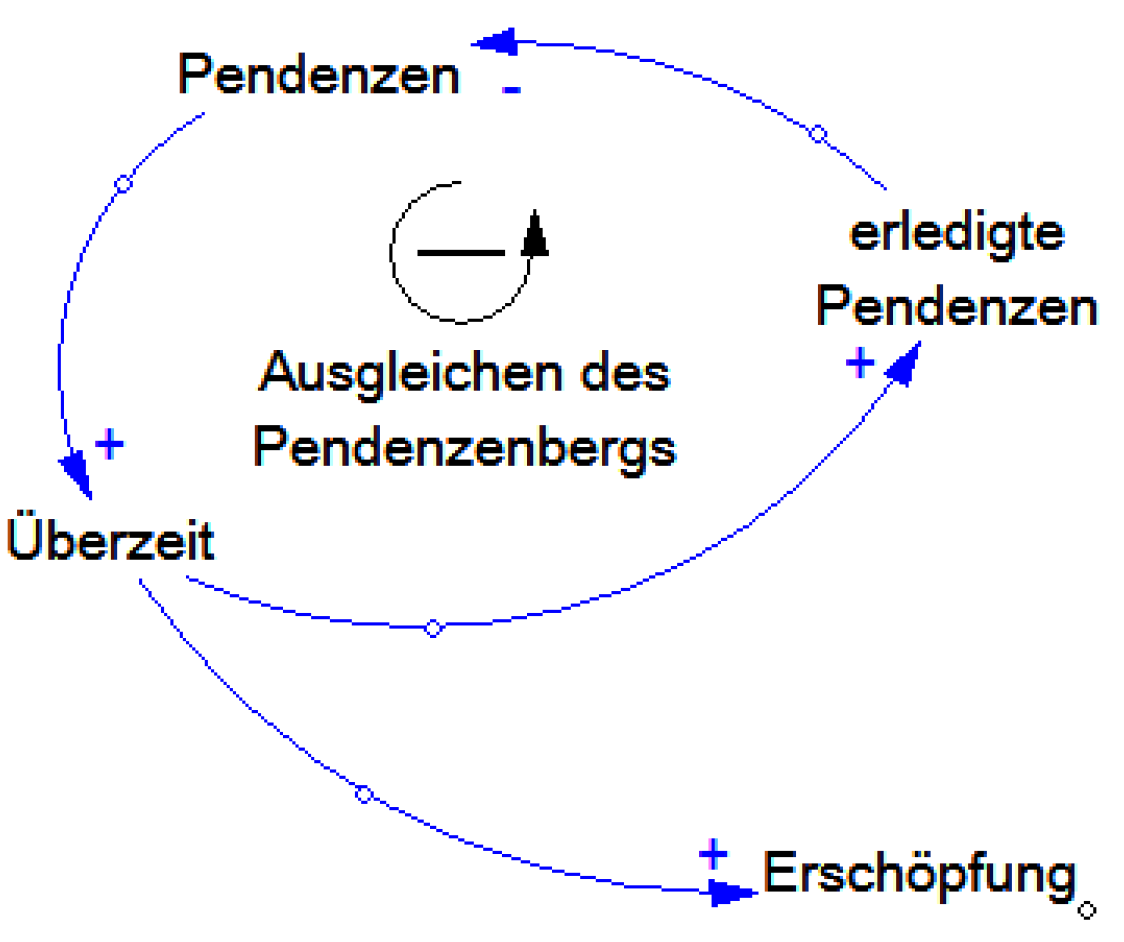
\includegraphics[width=0.225\textwidth]{pictures/regel_8_2}
		\item (Kausalbeziehungen) Markieren Sie wichtige Zeitverzögerungen mit // \\
		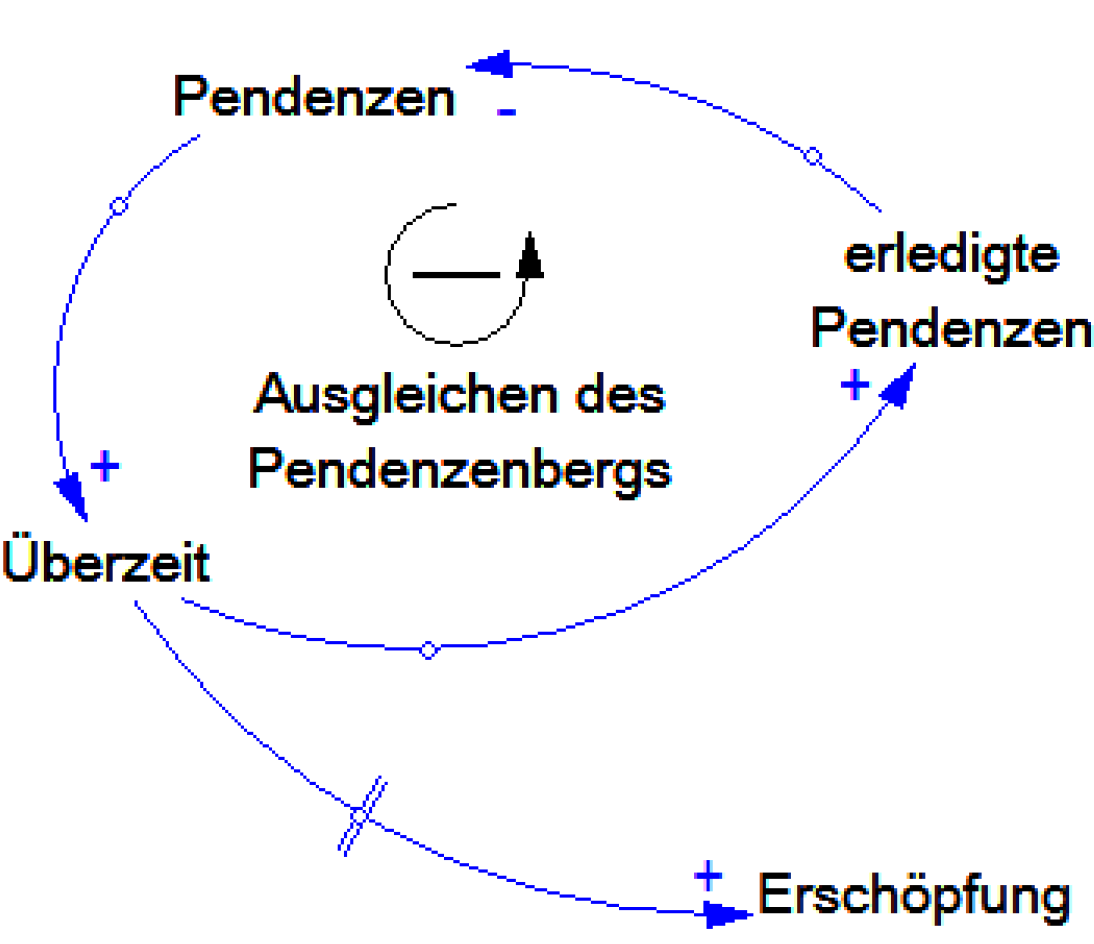
\includegraphics[width=0.225\textwidth]{pictures/regel_9}
		\item (Loops) ... und schliessen Sie die Loops \\
		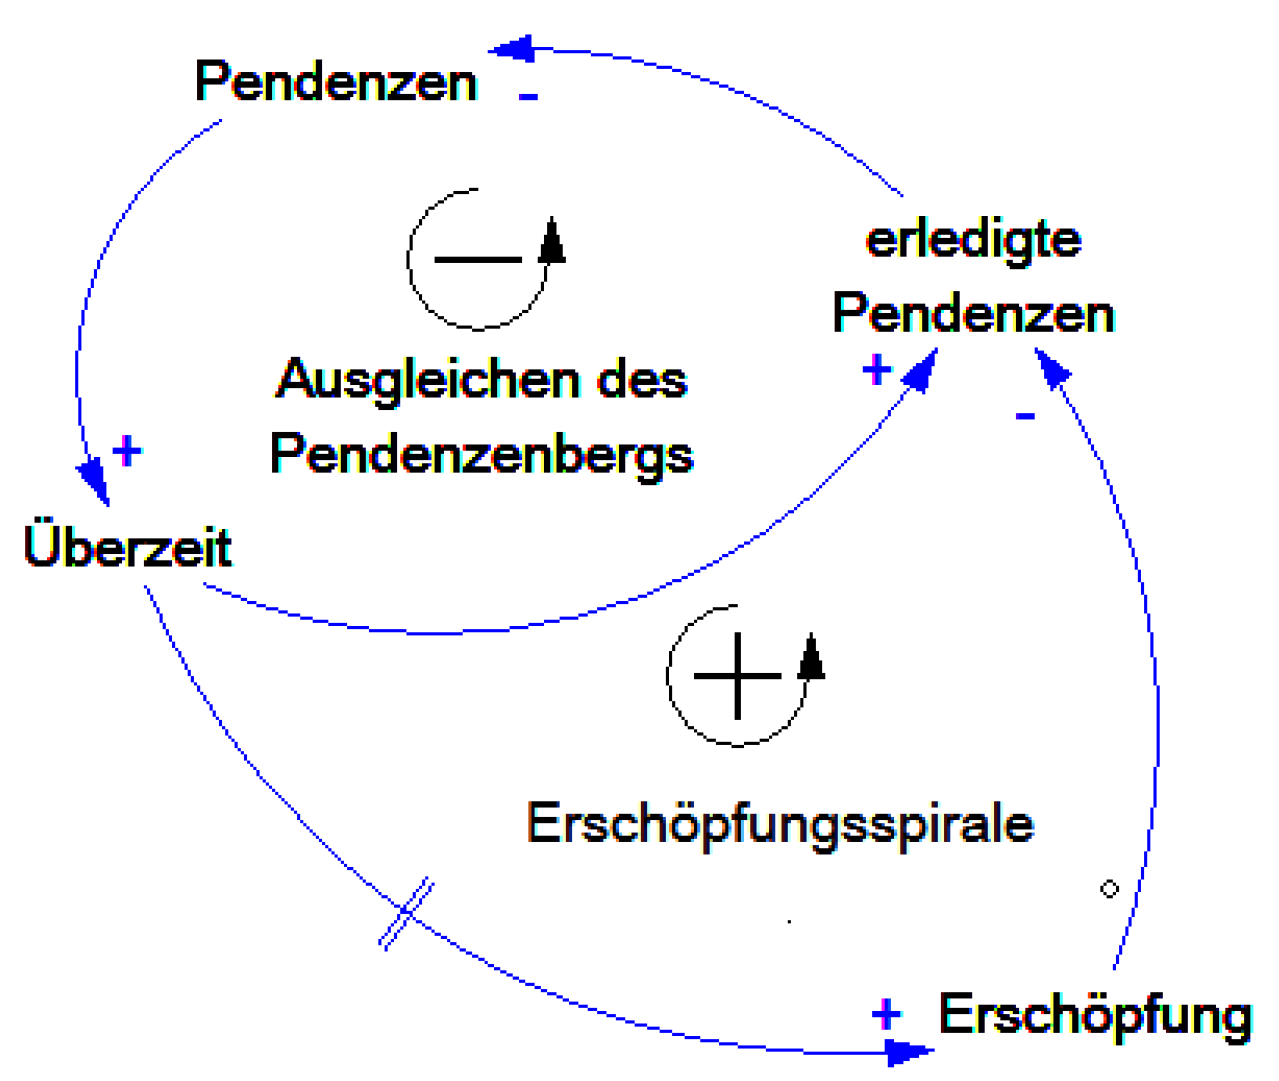
\includegraphics[width=0.225\textwidth]{pictures/regel_10}
		\item (Loops) Validieren Sie Rückkoppelungen: Welche Geschichte erzählt ein	Loop? Plausibilisieren Sie die mathematische Polarität eines Loops mit Ihrer Geschichte. \\
		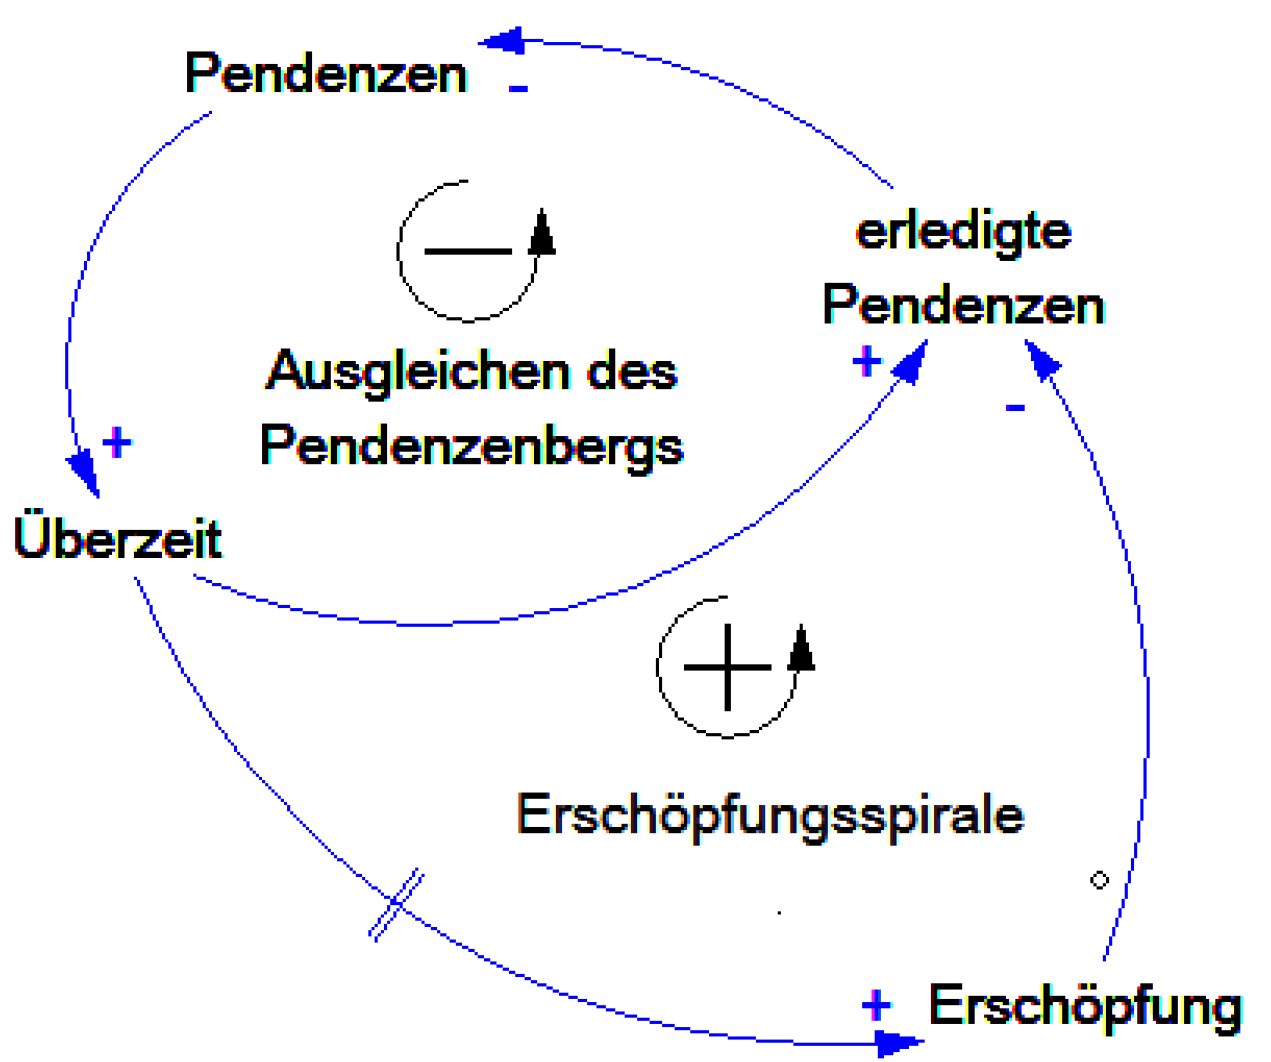
\includegraphics[width=0.225\textwidth]{pictures/regel_11}
		\item (Gesamtmodell) Fokussieren Sie auf den Modellzweck:
		\begin{compactitem}
			\item Welche Zielgrössen müssen zwingend modelliert werden?
			\item Welche Geschichten sind Ihnen - und anderen beteiligten Personen - besonders wichtig?
		\end{compactitem}
	\end{compactenum}
\end{multicols}	

\subsubsection{Verhaltensmuster}
Dynamische Systeme zeigen oftmals eines der folgenden charakteristischen Verhaltensmuster auf:
\begin{multicols}{3}
	\textbf{Exponentielles Wachstum (exponential growth):} \\
	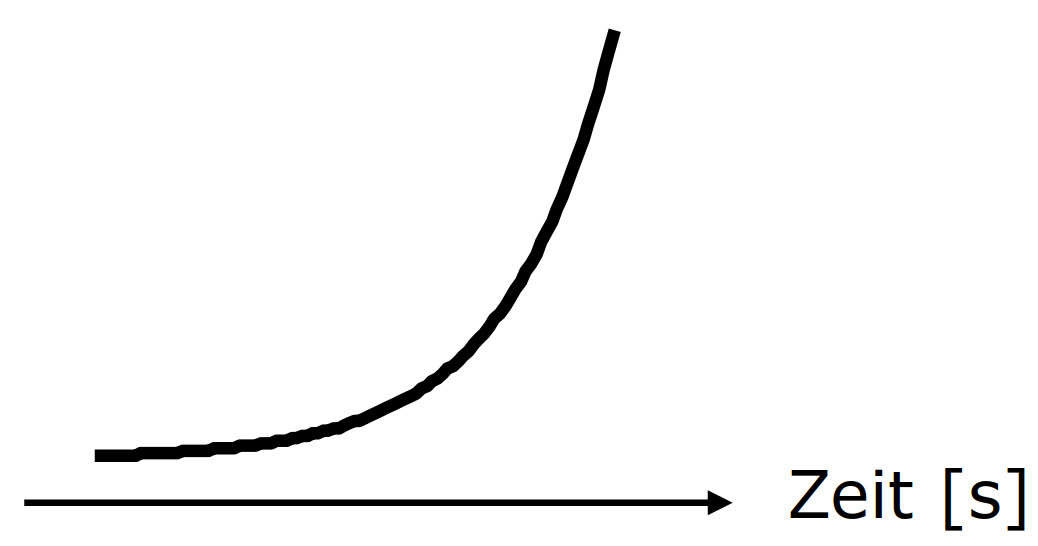
\includegraphics[width=0.3\textwidth]{pictures/verhalten_1} \\
	\textbf{Nach einem Ziel strebend (goal seeking):} \\
	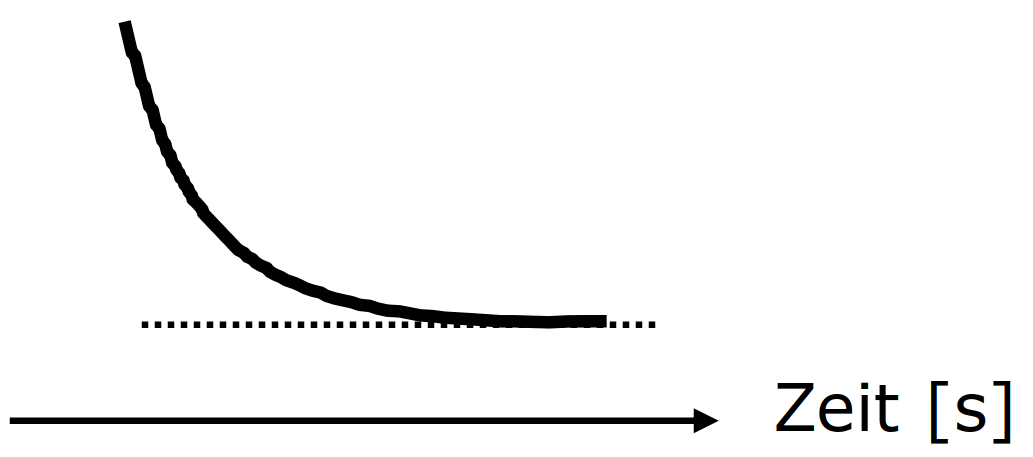
\includegraphics[width=0.3\textwidth]{pictures/verhalten_2} \\ \\
	\textbf{Oszillation (oscillation):} \\
	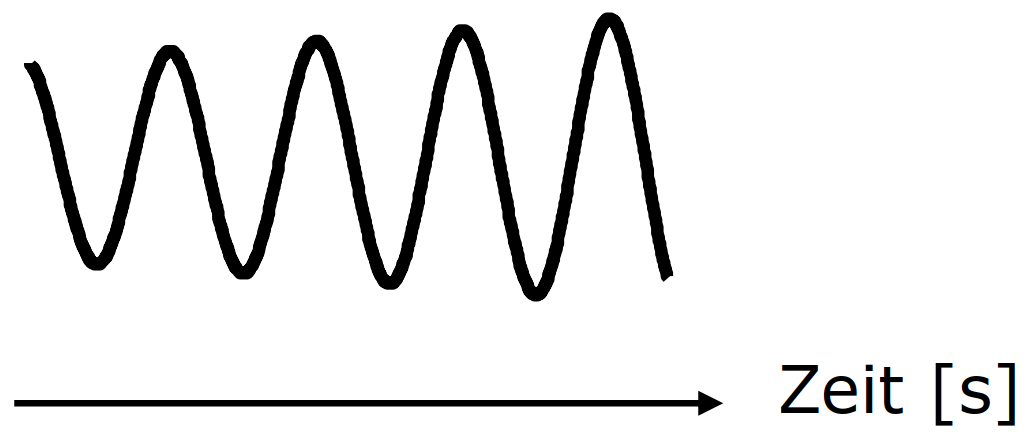
\includegraphics[width=0.3\textwidth]{pictures/verhalten_3}
\end{multicols}	
\begin{multicols}{3}
	\textbf{S-Kurve (S-shaped growth):} \\
	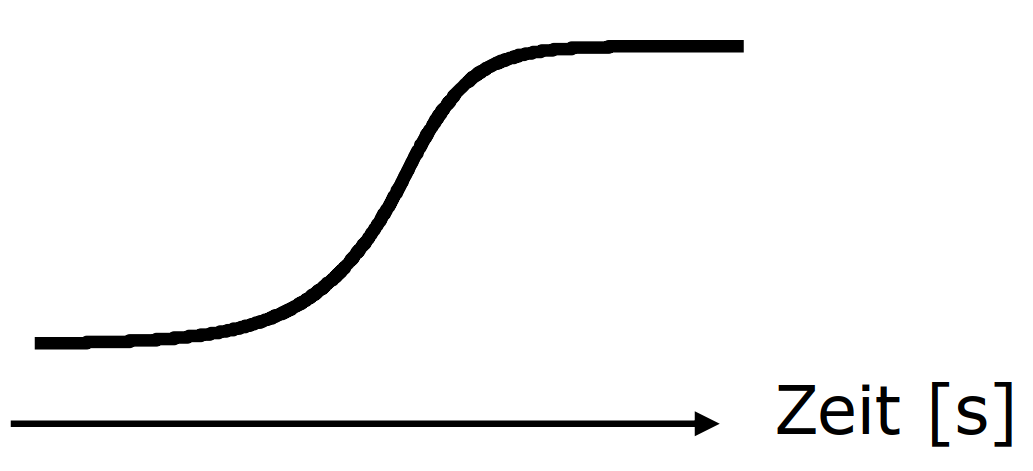
\includegraphics[width=0.3\textwidth]{pictures/verhalten_4} \\ \\
	\textbf{Wachstum mit Überschiessen (growth with overshoot):} \\
	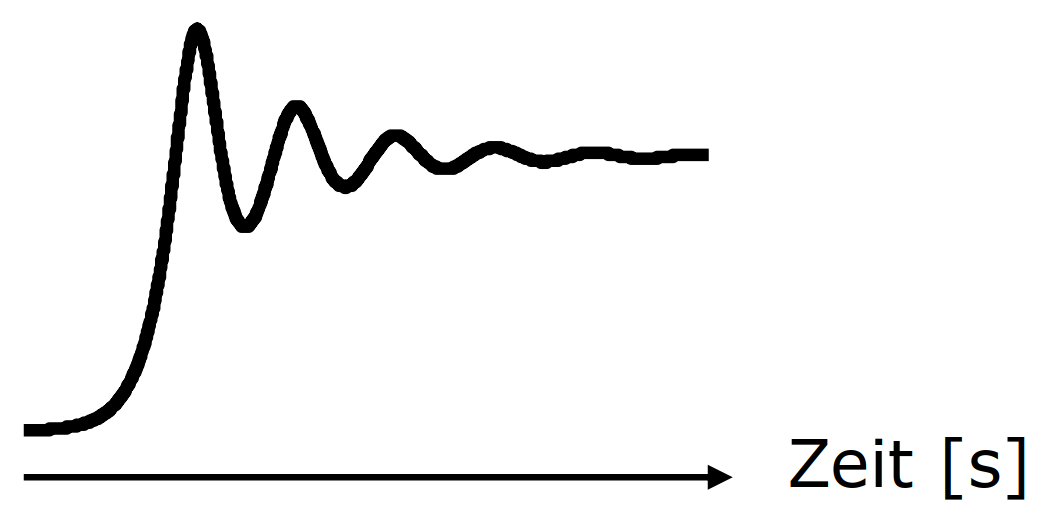
\includegraphics[width=0.3\textwidth]{pictures/verhalten_5} \\
	\textbf{Überschiessen und Kollaps (overshoot and collapse):} \\
	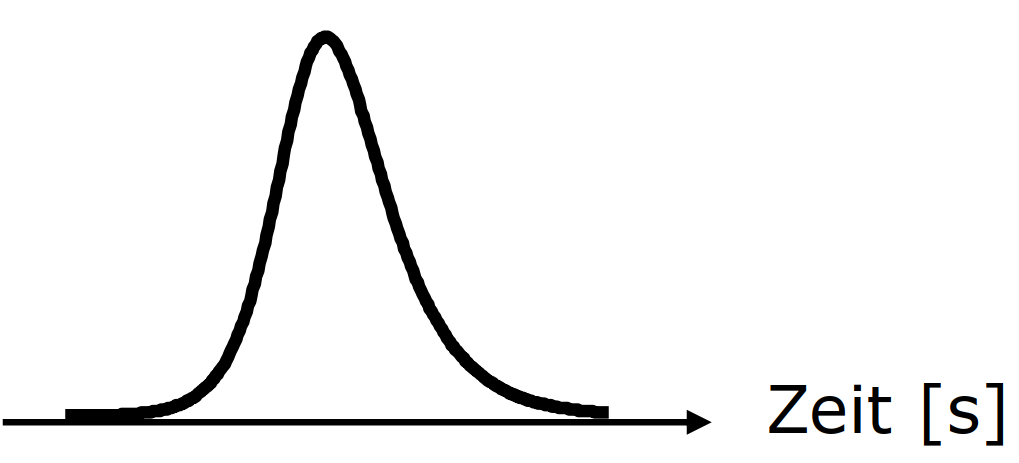
\includegraphics[width=0.3\textwidth]{pictures/verhalten_6} 
\end{multicols}	

\subsubsection{Strukturen Verhaltensmuster}
\begin{multicols}{2}
	\textbf{Exponentielles Wachstum:} \\
	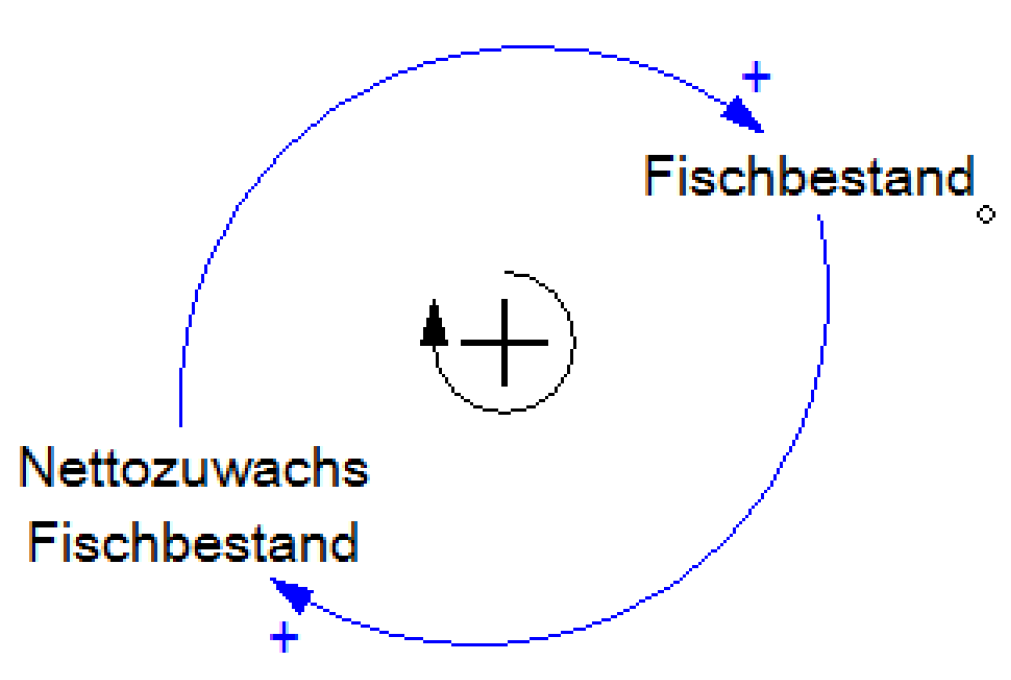
\includegraphics[width=0.3\textwidth]{pictures/struktur_1} \\ 
	\textbf{Nach einem Ziel strebend:} \\
	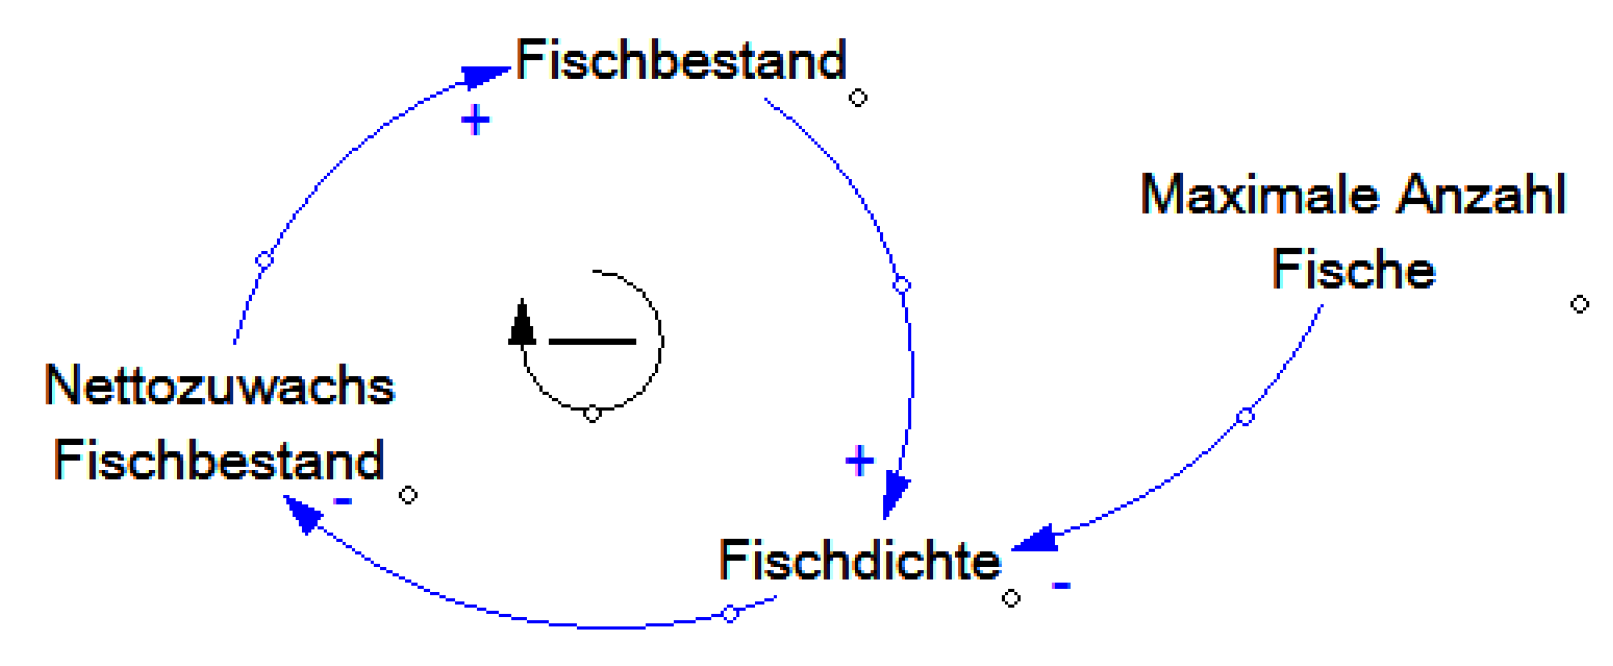
\includegraphics[width=0.45\textwidth]{pictures/struktur_2} 
\end{multicols}	
\begin{multicols}{2}
	\textbf{Oszillation:} \\
	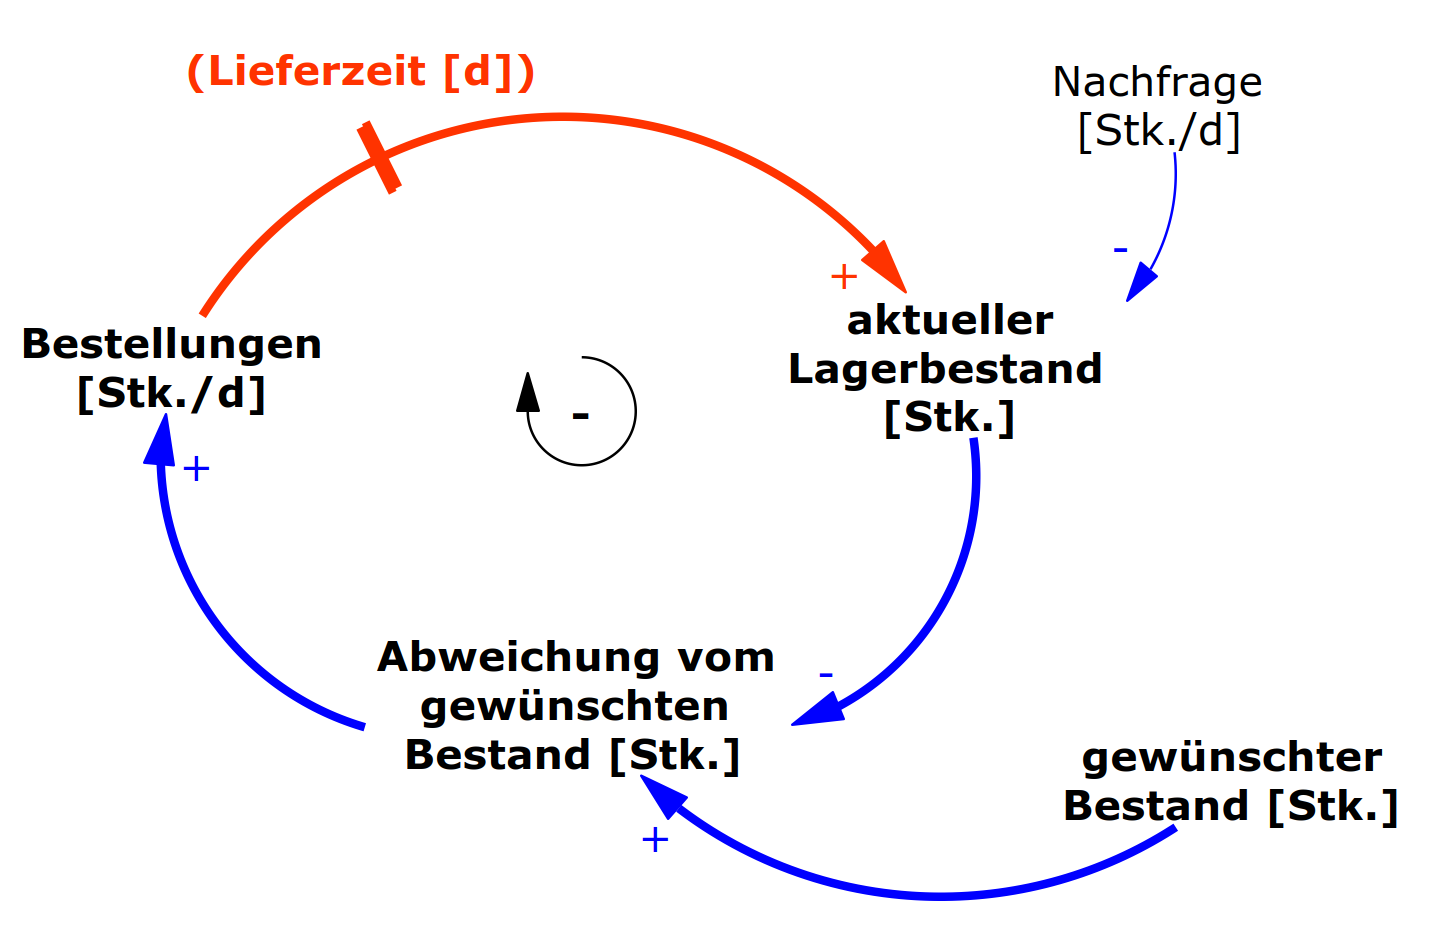
\includegraphics[width=0.3\textwidth]{pictures/struktur_3} \\
	\textbf{S-Kurve:} \\
	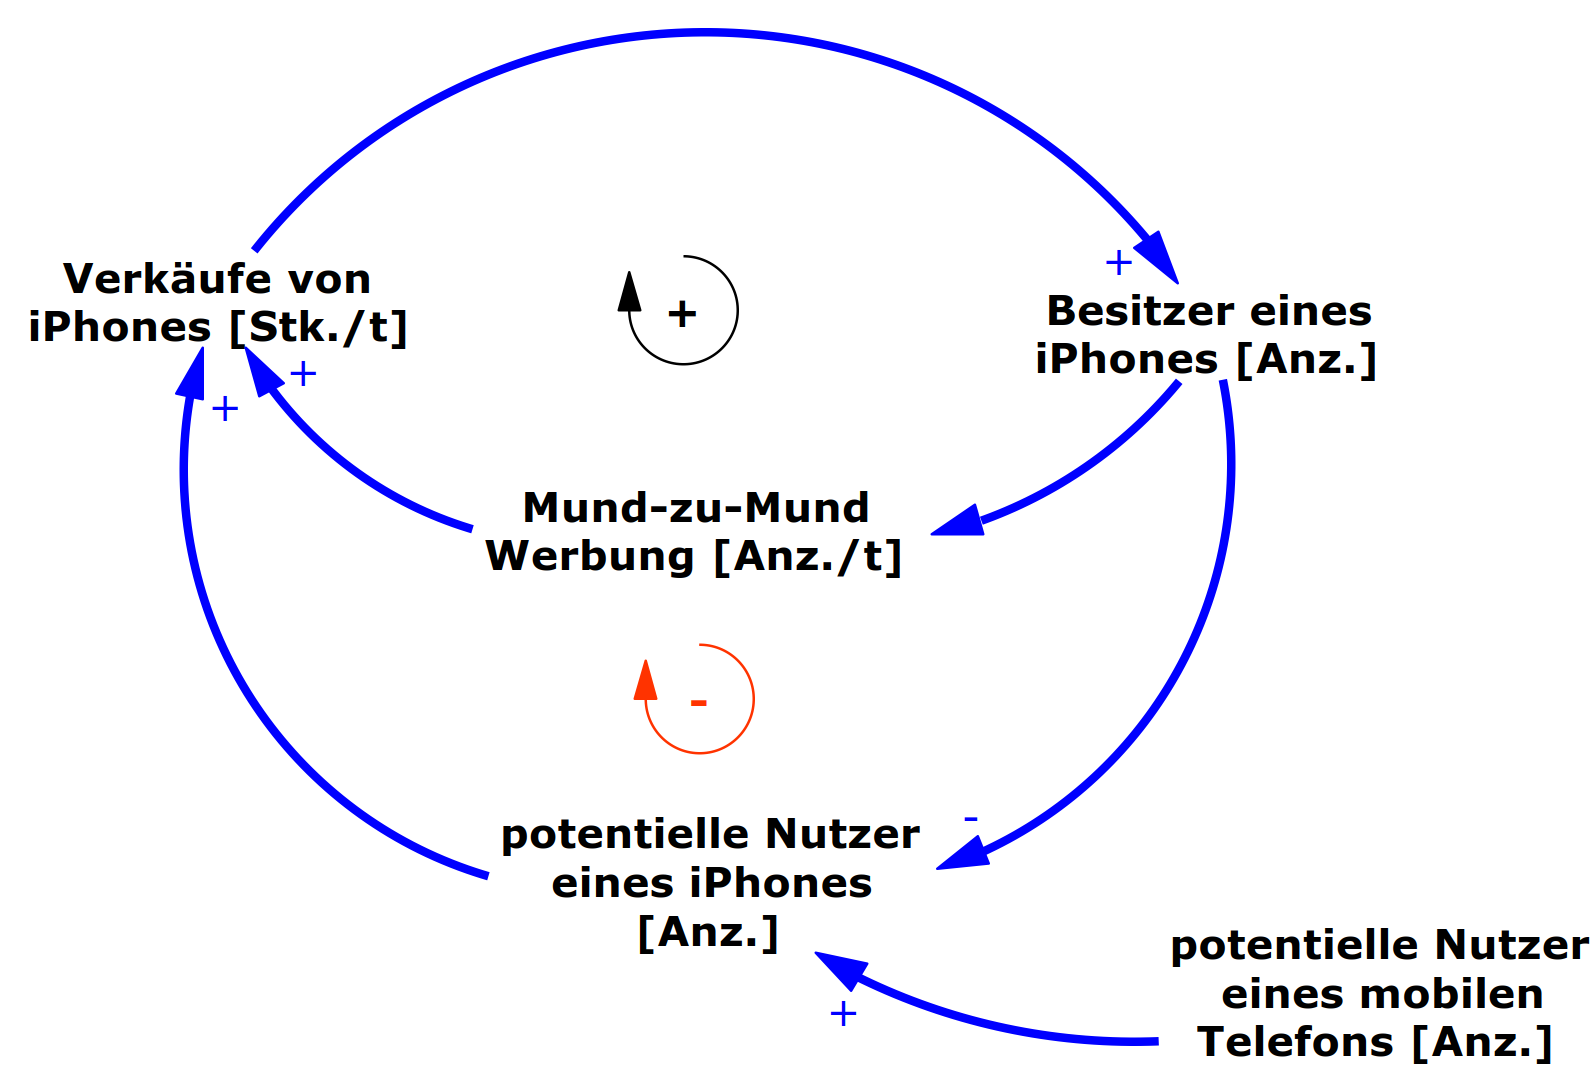
\includegraphics[width=0.3\textwidth]{pictures/struktur_4} 
\end{multicols}	
\begin{multicols}{2}
	\textbf{Wachstum mit Überschiessen:} \\
	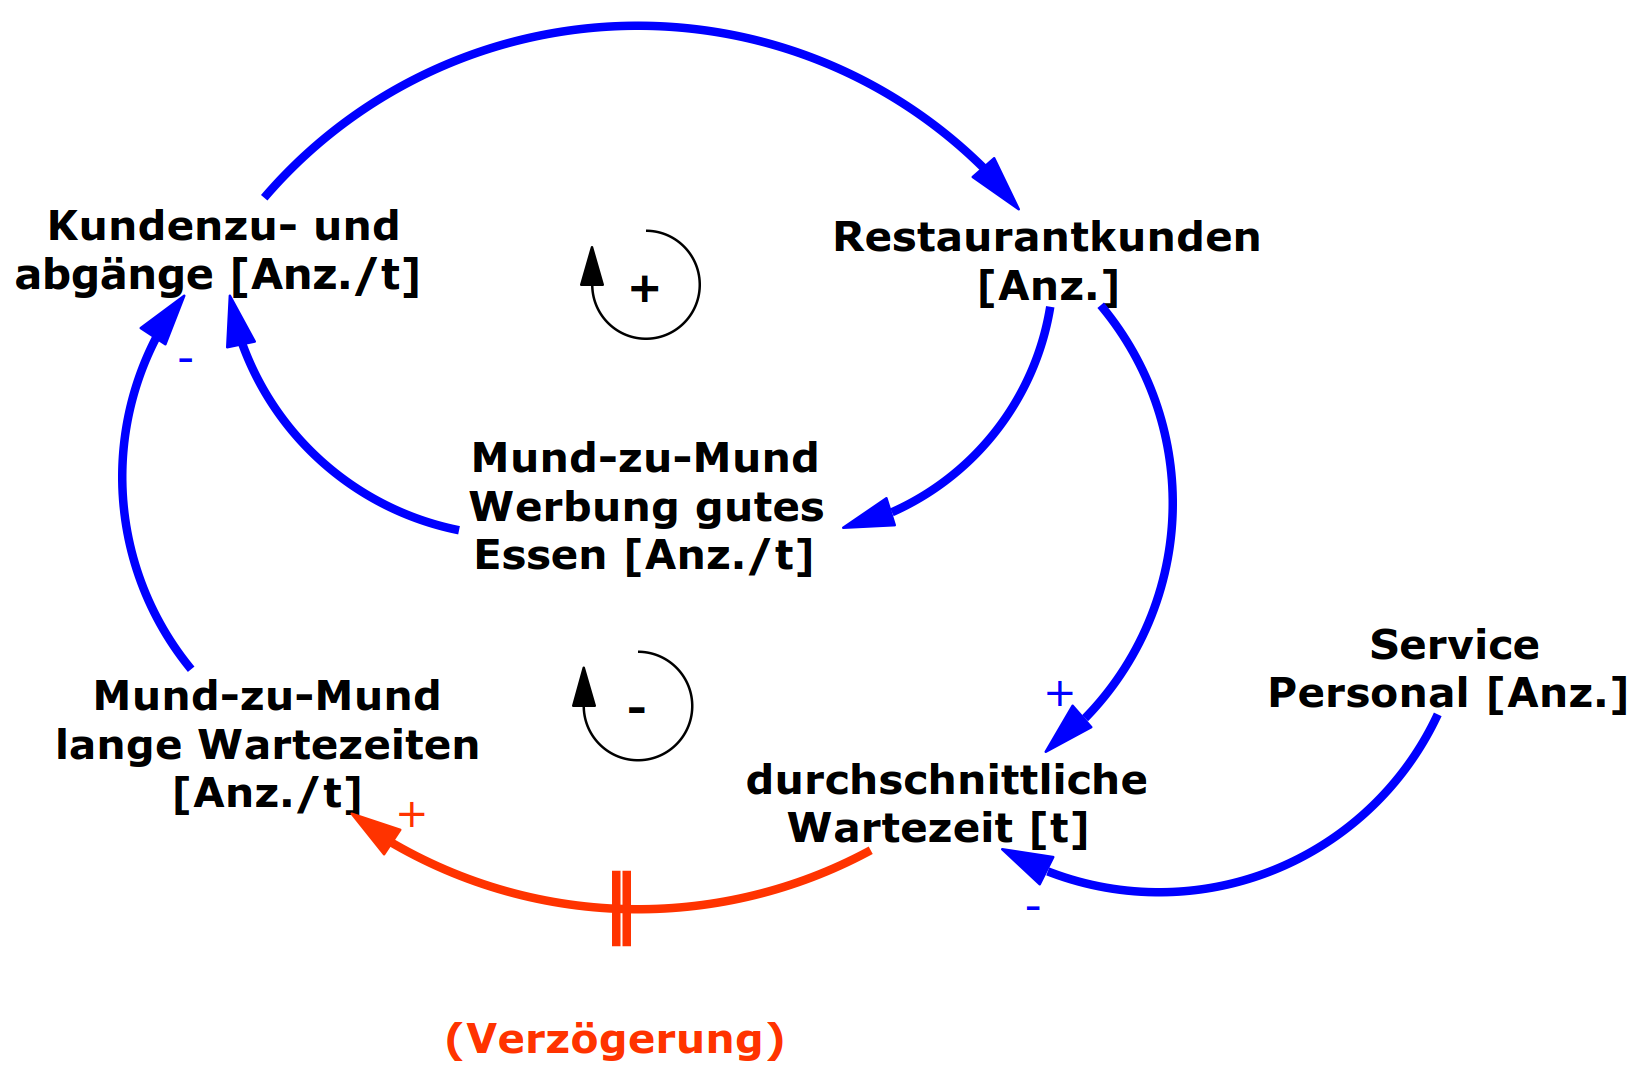
\includegraphics[width=0.3\textwidth]{pictures/struktur_5} \\ \\
	\textbf{Überschiessen und Kollaps:} \\
	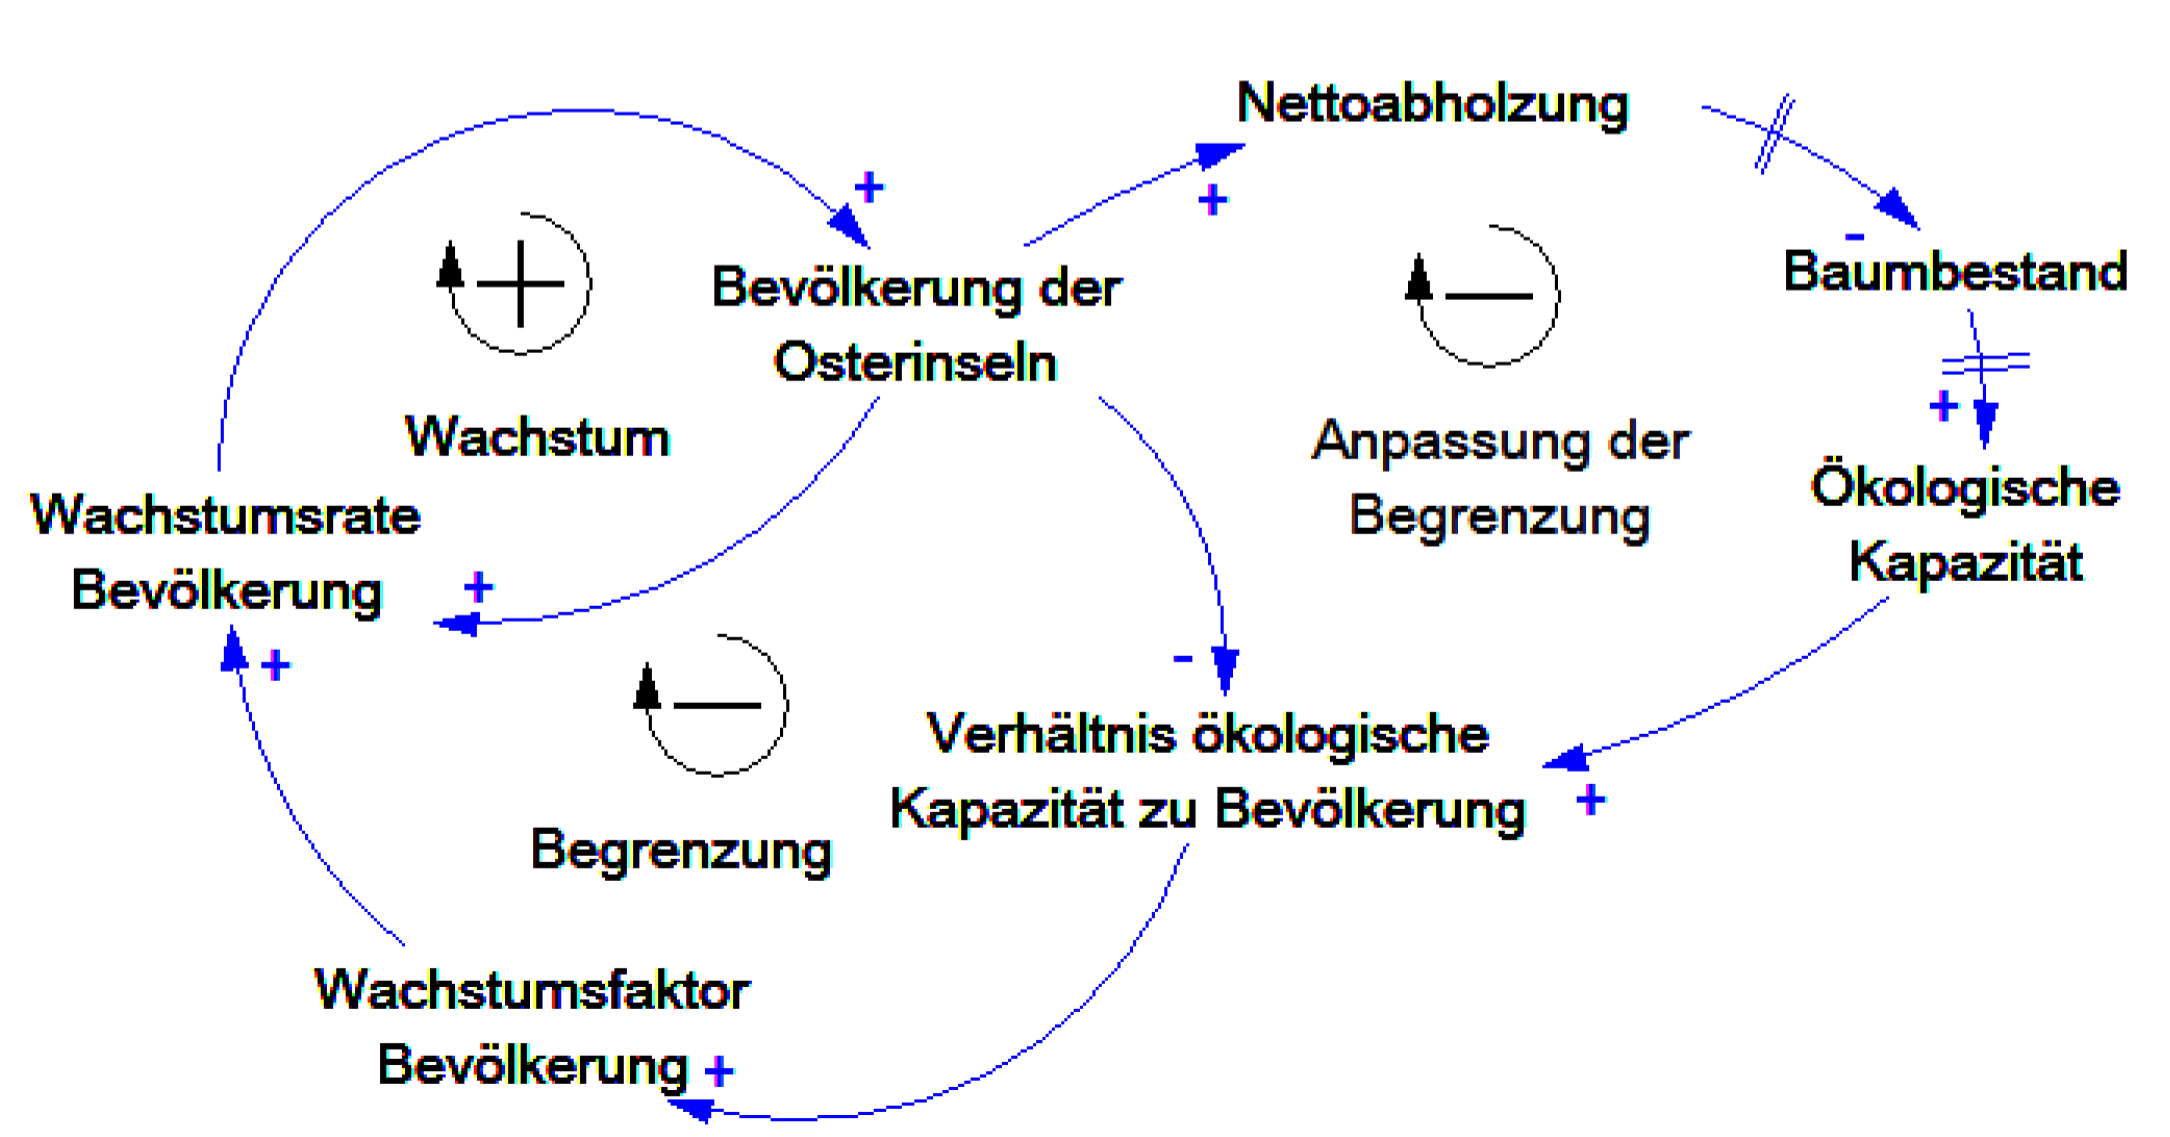
\includegraphics[width=0.45\textwidth]{pictures/struktur_6} 
\end{multicols}	

\subsubsection{System-Archetypen}
Muster und Strukturen, die in verschiedenen Kontexten in ähnlicher Weise auftreten.\\
\textbf{Vorteil}: Muster erkennen hilft relevante Dynamik-Probleme zu identifizieren.\\
\textbf{Achtung}: Real-World-Probleme benötigen trotzdem noch eine sorgfältige, spezifische Untersuchung.\\
\begin{multicols}{3}
	\textbf{Prozess balancieren mit Verzögerung (balancing process with delay):}\\
	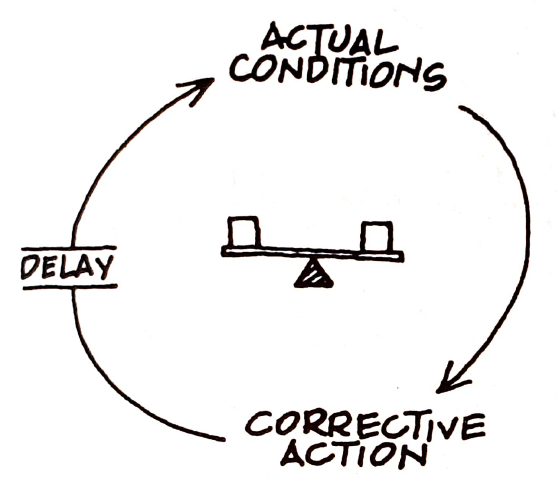
\includegraphics[width=0.8\linewidth]{pictures/archetype1}\\
	\vfill\null
	\columnbreak
	\textbf{Limiten beim Wachstum (limits to growth):}\\
	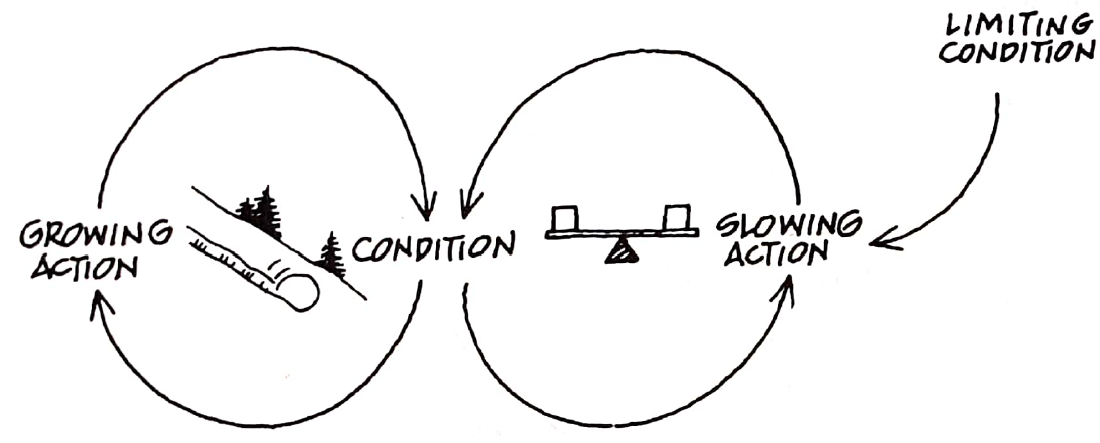
\includegraphics[width=\linewidth]{pictures/archetype2}\\
	\vfill\null
	\columnbreak
	\textbf{Fehlgeschlagene Lösungen (fixes that fail):}\\
	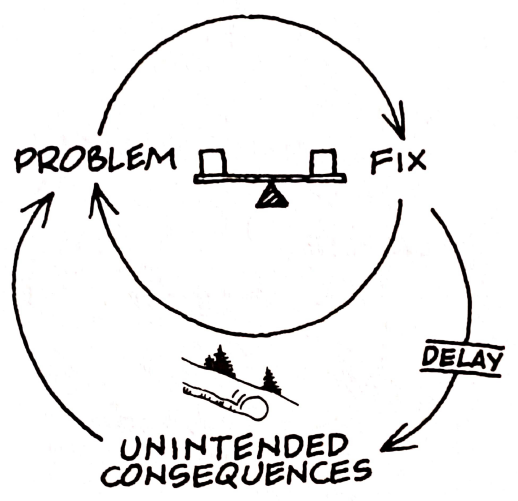
\includegraphics[width=0.8\linewidth]{pictures/archetype3}\\\
\end{multicols}
\begin{multicols}{3}
	\textbf{Verlagerung der Last (shifting the burden):}\\
	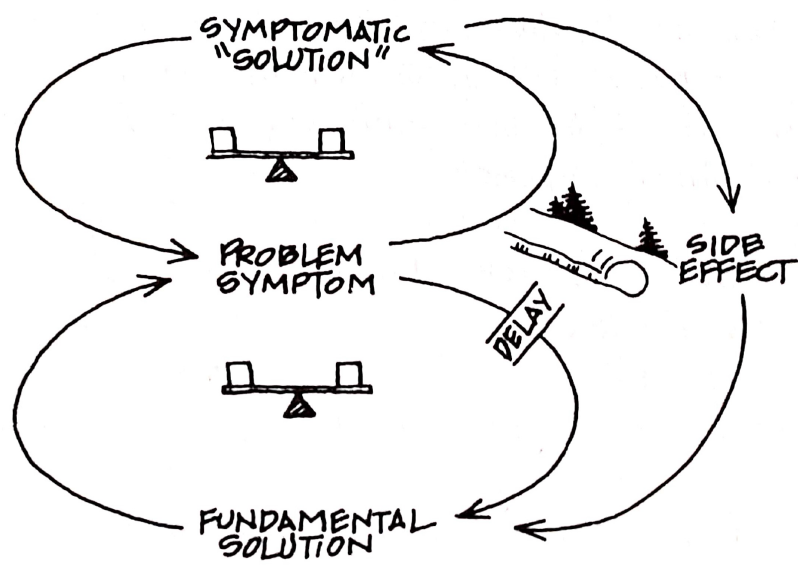
\includegraphics[width=\linewidth]{pictures/archetype4}\\
	\vfill\null
	\columnbreak
	\textbf{Erodierende Ziele (eroding goals)}\\
	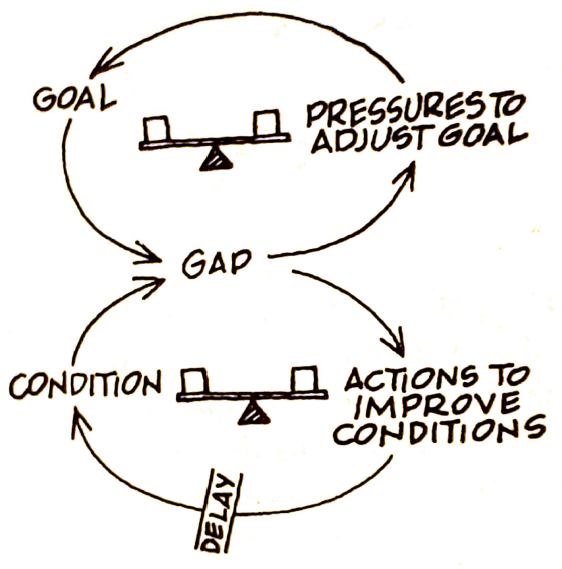
\includegraphics[width=0.8\linewidth]{pictures/archetype5}\\
	\vfill\null
	\columnbreak
	\textbf{Eskalation (escalation):}\\
	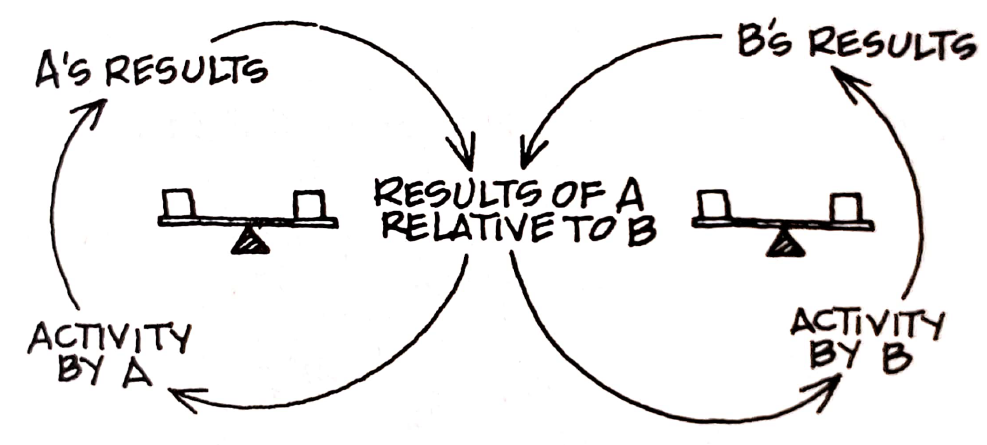
\includegraphics[width=\linewidth]{pictures/archetype6}\\
\end{multicols}
\begin{multicols}{3}
	\textbf{Tragödie der Gemeingüter (tragedy of the commons):}\\
	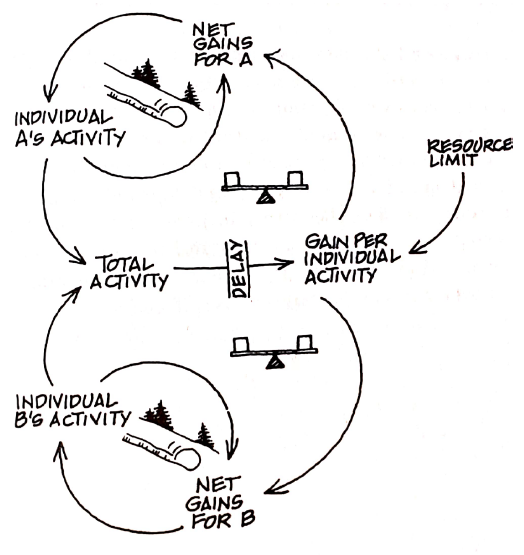
\includegraphics[width=\linewidth]{pictures/archetype7}\\
	\vfill\null
	\columnbreak
	\textbf{Wachstum und Unterfinanzierung (growth and underinvestment):}\\
	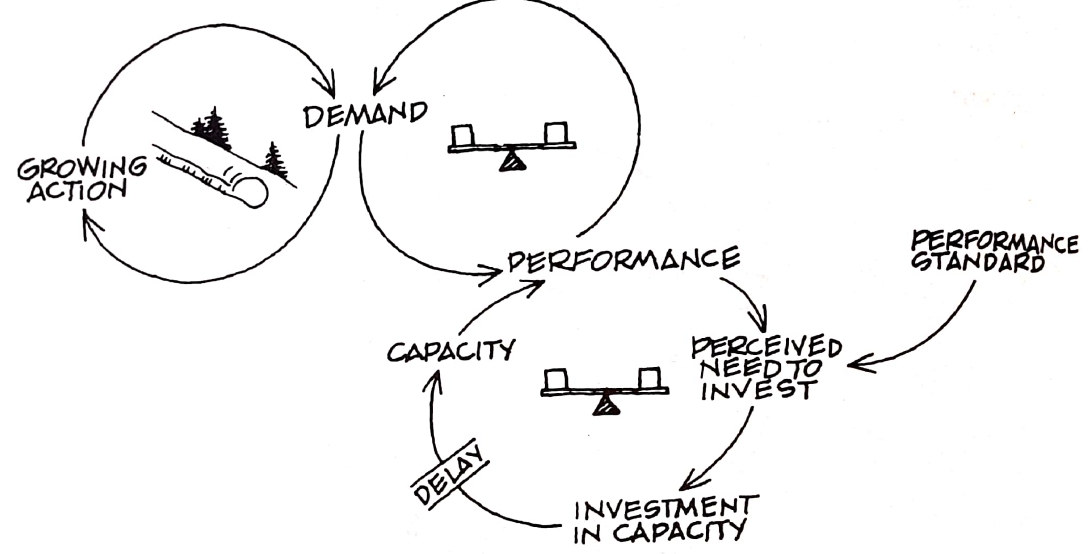
\includegraphics[width=\linewidth]{pictures/archetype8}\\
	\vfill\null
	\columnbreak
	\textbf{Erfolg den Erfolgreichen (success to the successful)}\\
	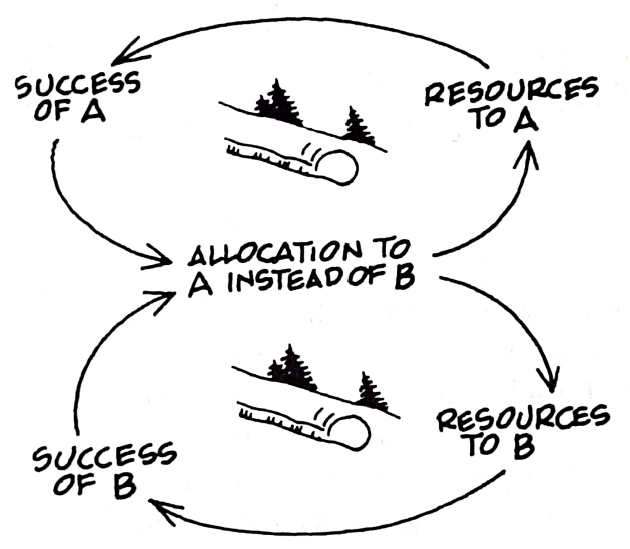
\includegraphics[width=0.8\linewidth]{pictures/archetype9}\\
\end{multicols}

\subsubsection{Pfadabhängigkeit}
Ein Lock-in-Zustand liegt vor, wenn
\begin{compactitem}
	\item auf Grund von Entscheidungen in der Vergangenheit
	\item eine Änderung der aktuellen Situation mit hohen Kosten verbunden ist und
	\item und deshalb oft unterbleibt.
\end{compactitem}
\begin{example}
	\begin{compactitem}
		\item billige Drucker und teure Farbpatronen
		\item Bonussysteme, Coop bis Lufthansa
		\item Beim Kauf eines Instruments wird die vorgängig bezahlte Miete teilweise angerechnet
	\end{compactitem}
\end{example}
\textbf{Linearer Polya-Prozess:} \\
\begin{tikzpicture}[node distance = 0.6cm and 0.5cm]	
	\node (n1) [decisionW] {Holzkugel ziehen};
	\node (n2) [decisionW, right=of n1] {Holzkugel zurücklegen und Holzkugel der gleichen Farbe	dazulegen};
	\draw [arrow] (n1) -- (n2);
	\draw [arrow] (n2.north) to[bend right] (n1.north);
\end{tikzpicture} \\
In einer Urne befinden sich eine blaue und eine grüne Kugel. Es wird blind eine Kugel herausgezogen. Die Wahrscheinlichkeit zur Ziehung einer Farbe beträgt 0.5. Die gezogene Kugel wird wieder zurückgelegt. Es wird nun eine weitere Kugel, welche die Farbe der soeben gezogenen aufweist, hinzugefügt. Es befindet sich nun eine Kugel mehr in der Urne als vor dem Zug. Wurde demnach eine blaue Kugel gezogen, beträgt die Wahrscheinlichkeit für die erneute Ziehung einer blauen Kugel 0.66. Dieser Vorgang ist pfadabhängig, da die Wahrscheinlichkeit, eine Kugel zu ziehen, welche eine gewünschte Farbe aufweist, mit der Anzahl an Kugeln jener Farbe zusammenhängt. Bereits der erste Zug hat eine hohe Relevanz, da die Anzahl an Kugeln evtl. noch gering ist und das Ziehen und das darauffolgende Hinzufügen einer Kugel auf den späteren Verlauf signifikante Auswirkungen hat. \\
\textbf{Lock-in Situation:}
\begin{compactitem}
	\item Ein und dasselbe System ist in unterschiedlichen Phasen sehr unterschiedlich empfindlich auf Störungen/Beeinflussungen.
	\item Bei bestimmten Systemzuständen reicht eine minimale Einflussnahme, um das	System in die gewünschte Richtung zu	beeinflussen. Solche Zustände liegen oft zu Beginn einer Entwicklung.
	\item In anderen Systemzuständen (meist später,	nach längerer Entwicklung), kann das System	nur noch mit grösstem Aufwand aus diesem Zustand gekippt werden (hohe Investition).
\end{compactitem}